\section{Results for \MtName{} against Reader v2 and Reader v3}\label{sec:results-Mt}

\MtName{} is the checkpoint at the end of stage s2 of the chain (stages s1, ft116k and s2). Table~\ref{tab:cmp-Mt-Three} gives for all fourteen units, in three blocks, three measures of Reader v3 and \MtName{} (the AUC, the AUC on thin strokes and false ink at 80 per cent recall) and, under the units, the mean and the median of each measure over the fourteen units; Table~\ref{tab:cmp-Mt-Two} gives the same for Reader v2 and \MtName{}. The text below gives, for the eight held-out units, the mean, the median and the number of units on which \MtName{} scores above each reader in AUC.

\begin{table*}[!t]
\caption{Three measures of \MtName{} against Reader v3 on the fourteen units: the AUC, the AUC on thin
strokes and false ink at 80 per cent recall. The cell of \MtName{} gives in parentheses the signed difference
against Reader v3. The rows Mean and Median are taken over all fourteen units; the
block of the community labels is information only.}\label{tab:cmp-Mt-Three}
\centering
\definecolor{rgreen}{RGB}{46,139,74}\definecolor{rred}{RGB}{192,57,43}
{\small\setlength{\tabcolsep}{2.2pt}
\noindent\begin{tabular}{>{\raggedright\arraybackslash}p{3.0cm}>{\raggedleft\arraybackslash}p{1.5cm}>{\raggedleft\arraybackslash}p{3.0cm}>{\raggedleft\arraybackslash}p{1.5cm}>{\raggedleft\arraybackslash}p{3.0cm}>{\raggedleft\arraybackslash}p{1.5cm}>{\raggedleft\arraybackslash}p{3.0cm}}
\hline
unit & \multicolumn{2}{c}{AUC} & \multicolumn{2}{c}{\shortstack{AUC on\\thin strokes}} & \multicolumn{2}{c}{\shortstack{false ink at 80\\per cent recall}} \\
 & {\footnotesize Reader v3} & {\footnotesize Rectina m3} & {\footnotesize Reader v3} & {\footnotesize Rectina m3} & {\footnotesize Reader v3} & {\footnotesize Rectina m3} \\
\hline
\multicolumn{7}{@{}p{\dimexpr 16.5cm+30.8pt\relax}@{}}{\rule{0pt}{2.6ex}\textit{Control units outside the training segments, organisers' labels: 0343 (approved letters, 116 keV); 0841 (113 keV)}} \\
0343 & \textbf{0.9078} & \textcolor{rred}{$\blacktriangledown$}\,0.8911 {\scriptsize (-0.0168)} & \textbf{0.9246} & \textcolor{rred}{$\blacktriangledown$}\,0.9104 {\scriptsize (-0.0142)} & \textbf{0.0690} & \textcolor{rred}{$\blacktriangledown$}\,0.0865 {\scriptsize (+0.0175)} \\
0841 ag1 & 0.8513 & \textcolor{rgreen}{$\blacktriangle$}\,\textbf{0.8532} {\scriptsize (+0.0019)} & 0.8648 & \textcolor{rgreen}{$\blacktriangle$}\,\textbf{0.8685} {\scriptsize (+0.0038)} & \textbf{0.2153} & \textcolor{rred}{$\blacktriangledown$}\,0.2240 {\scriptsize (+0.0087)} \\
0841 ag2 & 0.8297 & \textcolor{rgreen}{$\blacktriangle$}\,\textbf{0.8390} {\scriptsize (+0.0093)} & 0.8474 & \textcolor{rgreen}{$\blacktriangle$}\,\textbf{0.8563} {\scriptsize (+0.0090)} & \textbf{0.2681} & \textcolor{rred}{$\blacktriangledown$}\,0.2744 {\scriptsize (+0.0063)} \\
0841 w00 & \textbf{0.9055} & \textcolor{rred}{$\blacktriangledown$}\,0.8723 {\scriptsize (-0.0331)} & \textbf{0.9221} & \textcolor{rred}{$\blacktriangledown$}\,0.8941 {\scriptsize (-0.0280)} & \textbf{0.1444} & \textcolor{rred}{$\blacktriangledown$}\,0.2078 {\scriptsize (+0.0634)} \\
\multicolumn{7}{@{}p{\dimexpr 16.5cm+30.8pt\relax}@{}}{\rule{0pt}{2.6ex}\textit{Control units outside the training segments, community labels, information only: 1447 (116 keV)}} \\
1447 w058 & \textbf{0.8610} & \textcolor{rred}{$\blacktriangledown$}\,0.8520 {\scriptsize (-0.0090)} & \textbf{0.8965} & \textcolor{rred}{$\blacktriangledown$}\,0.8865 {\scriptsize (-0.0100)} & 0.2665 & \textcolor{rgreen}{$\blacktriangle$}\,\textbf{0.2637} {\scriptsize (-0.0028)} \\
1447 w060 & \textbf{0.7842} & \textcolor{rred}{$\blacktriangledown$}\,0.7777 {\scriptsize (-0.0065)} & \textbf{0.8276} & \textcolor{rred}{$\blacktriangledown$}\,0.8171 {\scriptsize (-0.0105)} & \textbf{0.4095} & \textcolor{rred}{$\blacktriangledown$}\,0.4130 {\scriptsize (+0.0035)} \\
\multicolumn{7}{@{}p{\dimexpr 16.5cm+30.8pt\relax}@{}}{\rule{0pt}{2.6ex}\textit{Held-out segments of training scrolls, our validation labels: 0009B and 0343P (116 keV), 0500P2 (113 keV)}} \\
0009B$\cdot$172639 & 0.8456 & \textcolor{rgreen}{$\blacktriangle$}\,\textbf{0.8909} {\scriptsize (+0.0453)} & 0.8515 & \textcolor{rgreen}{$\blacktriangle$}\,\textbf{0.8955} {\scriptsize (+0.0439)} & 0.3114 & \textcolor{rgreen}{$\blacktriangle$}\,\textbf{0.1704} {\scriptsize (-0.1410)} \\
0009B$\cdot$125754 & \textbf{0.9562} & \textcolor{rred}{$\blacktriangledown$}\,0.9454 {\scriptsize (-0.0107)} & \textbf{0.9636} & \textcolor{rred}{$\blacktriangledown$}\,0.9550 {\scriptsize (-0.0086)} & \textbf{0.0460} & \textcolor{rred}{$\blacktriangledown$}\,0.0681 {\scriptsize (+0.0221)} \\
0009B$\cdot$133208 & 0.8551 & \textcolor{rgreen}{$\blacktriangle$}\,\textbf{0.8658} {\scriptsize (+0.0107)} & 0.8672 & \textcolor{rgreen}{$\blacktriangle$}\,\textbf{0.8775} {\scriptsize (+0.0103)} & 0.2774 & \textcolor{rgreen}{$\blacktriangle$}\,\textbf{0.2382} {\scriptsize (-0.0392)} \\
0009B$\cdot$140325 & \textbf{0.9040} & \textcolor{rred}{$\blacktriangledown$}\,0.8761 {\scriptsize (-0.0278)} & \textbf{0.9110} & \textcolor{rred}{$\blacktriangledown$}\,0.8857 {\scriptsize (-0.0253)} & \textbf{0.1574} & \textcolor{rred}{$\blacktriangledown$}\,0.2171 {\scriptsize (+0.0596)} \\
0500P2$\cdot$055229 & \textbf{0.8971} & \textcolor{rred}{$\blacktriangledown$}\,0.8479 {\scriptsize (-0.0491)} & \textbf{0.9074} & \textcolor{rred}{$\blacktriangledown$}\,0.8613 {\scriptsize (-0.0461)} & \textbf{0.1360} & \textcolor{rred}{$\blacktriangledown$}\,0.3089 {\scriptsize (+0.1729)} \\
0500P2$\cdot$055230 & \textbf{0.7881} & \textcolor{rred}{$\blacktriangledown$}\,0.7778 {\scriptsize (-0.0103)} & \textbf{0.7980} & \textcolor{rred}{$\blacktriangledown$}\,0.7882 {\scriptsize (-0.0098)} & 0.3998 & \textcolor{rgreen}{$\blacktriangle$}\,\textbf{0.3846} {\scriptsize (-0.0153)} \\
0343P$\cdot$233748-0 & 0.8340 & \textcolor{rgreen}{$\blacktriangle$}\,\textbf{0.8377} {\scriptsize (+0.0037)} & 0.8398 & \textcolor{rgreen}{$\blacktriangle$}\,\textbf{0.8435} {\scriptsize (+0.0037)} & 0.3059 & \textcolor{rgreen}{$\blacktriangle$}\,\textbf{0.2914} {\scriptsize (-0.0145)} \\
0343P$\cdot$172054-1 & 0.7573 & \textcolor{rgreen}{$\blacktriangle$}\,\textbf{0.7838} {\scriptsize (+0.0264)} & 0.7669 & \textcolor{rgreen}{$\blacktriangle$}\,\textbf{0.7931} {\scriptsize (+0.0262)} & 0.4336 & \textcolor{rgreen}{$\blacktriangle$}\,\textbf{0.3870} {\scriptsize (-0.0466)} \\
\hline
Mean & \textbf{0.8555} & \textcolor{rred}{$\blacktriangledown$}\,0.8508 {\scriptsize (-0.0047)} & \textbf{0.8706} & \textcolor{rred}{$\blacktriangledown$}\,0.8666 {\scriptsize (-0.0040)} & \textbf{0.2458} & \textcolor{rred}{$\blacktriangledown$}\,0.2525 {\scriptsize (+0.0068)} \\
\hline
Median & \textbf{0.8532} & \textcolor{rred}{$\blacktriangledown$}\,0.8526 {\scriptsize (-0.0006)} & 0.8660 & \textcolor{rgreen}{$\blacktriangle$}\,\textbf{0.8730} {\scriptsize (+0.0070)} & 0.2673 & \textcolor{rgreen}{$\blacktriangle$}\,\textbf{0.2510} {\scriptsize (-0.0163)} \\
\hline
\end{tabular}}

\par\smallskip
{\footnotesize\raggedrightAUC: the rank AUC of ink against blank pixels. \\
AUC on thin strokes: the rank AUC of the central 80 per cent of each stroke against blank pixels at least 207 um from any label, the band between not scored. \\
false ink at 80 per cent recall: the share of blank pixels marked as ink at the threshold that recalls 80 per cent of the ink pixels, where less is better. \\
For the controls the AUC is taken against the far negatives of the bench; for the held-out units against all blank pixels of the validation mask. \\
The better value of each pair in bold; a green triangle pointing up before \MtName{} where it is better, a red triangle pointing down where it is worse. \\
A pair whose two values are equal at four decimals has no bold value and no triangle.
\par}
\end{table*}

\begin{table*}[!t]
\caption{Three measures of \MtName{} against Reader v2 on the fourteen units, in the format of Table~\ref{tab:cmp-Mt-Three}. The cell of \MtName{} gives in parentheses the signed difference
against Reader v2. The rows Mean and Median are taken over all fourteen units; the
block of the community labels is information only.}\label{tab:cmp-Mt-Two}
\centering
\definecolor{rgreen}{RGB}{46,139,74}\definecolor{rred}{RGB}{192,57,43}
{\small\setlength{\tabcolsep}{2.2pt}
\noindent\begin{tabular}{>{\raggedright\arraybackslash}p{3.0cm}>{\raggedleft\arraybackslash}p{1.5cm}>{\raggedleft\arraybackslash}p{3.0cm}>{\raggedleft\arraybackslash}p{1.5cm}>{\raggedleft\arraybackslash}p{3.0cm}>{\raggedleft\arraybackslash}p{1.5cm}>{\raggedleft\arraybackslash}p{3.0cm}}
\hline
unit & \multicolumn{2}{c}{AUC} & \multicolumn{2}{c}{\shortstack{AUC on\\thin strokes}} & \multicolumn{2}{c}{\shortstack{false ink at 80\\per cent recall}} \\
 & {\footnotesize Reader v2} & {\footnotesize Rectina m3} & {\footnotesize Reader v2} & {\footnotesize Rectina m3} & {\footnotesize Reader v2} & {\footnotesize Rectina m3} \\
\hline
\multicolumn{7}{@{}p{\dimexpr 16.5cm+30.8pt\relax}@{}}{\rule{0pt}{2.6ex}\textit{Control units outside the training segments, organisers' labels: 0343 (approved letters, 116 keV); 0841 (113 keV)}} \\
0343 & \textbf{0.8956} & \textcolor{rred}{$\blacktriangledown$}\,0.8911 {\scriptsize (-0.0045)} & \textbf{0.9136} & \textcolor{rred}{$\blacktriangledown$}\,0.9104 {\scriptsize (-0.0032)} & \textbf{0.0807} & \textcolor{rred}{$\blacktriangledown$}\,0.0865 {\scriptsize (+0.0058)} \\
0841 ag1 & 0.8410 & \textcolor{rgreen}{$\blacktriangle$}\,\textbf{0.8532} {\scriptsize (+0.0123)} & 0.8538 & \textcolor{rgreen}{$\blacktriangle$}\,\textbf{0.8685} {\scriptsize (+0.0147)} & 0.2379 & \textcolor{rgreen}{$\blacktriangle$}\,\textbf{0.2240} {\scriptsize (-0.0138)} \\
0841 ag2 & 0.8250 & \textcolor{rgreen}{$\blacktriangle$}\,\textbf{0.8390} {\scriptsize (+0.0140)} & 0.8431 & \textcolor{rgreen}{$\blacktriangle$}\,\textbf{0.8563} {\scriptsize (+0.0132)} & 0.2904 & \textcolor{rgreen}{$\blacktriangle$}\,\textbf{0.2744} {\scriptsize (-0.0160)} \\
0841 w00 & \textbf{0.8767} & \textcolor{rred}{$\blacktriangledown$}\,0.8723 {\scriptsize (-0.0043)} & \textbf{0.8964} & \textcolor{rred}{$\blacktriangledown$}\,0.8941 {\scriptsize (-0.0023)} & \textbf{0.1912} & \textcolor{rred}{$\blacktriangledown$}\,0.2078 {\scriptsize (+0.0166)} \\
\multicolumn{7}{@{}p{\dimexpr 16.5cm+30.8pt\relax}@{}}{\rule{0pt}{2.6ex}\textit{Control units outside the training segments, community labels, information only: 1447 (116 keV)}} \\
1447 w058 & \textbf{0.8575} & \textcolor{rred}{$\blacktriangledown$}\,0.8520 {\scriptsize (-0.0055)} & \textbf{0.8934} & \textcolor{rred}{$\blacktriangledown$}\,0.8865 {\scriptsize (-0.0069)} & 0.2689 & \textcolor{rgreen}{$\blacktriangle$}\,\textbf{0.2637} {\scriptsize (-0.0052)} \\
1447 w060 & 0.7777 & 0.7777 {\scriptsize (+0.0000)} & \textbf{0.8185} & \textcolor{rred}{$\blacktriangledown$}\,0.8171 {\scriptsize (-0.0015)} & 0.4240 & \textcolor{rgreen}{$\blacktriangle$}\,\textbf{0.4130} {\scriptsize (-0.0110)} \\
\multicolumn{7}{@{}p{\dimexpr 16.5cm+30.8pt\relax}@{}}{\rule{0pt}{2.6ex}\textit{Held-out segments of training scrolls, our validation labels: 0009B and 0343P (116 keV), 0500P2 (113 keV)}} \\
0009B$\cdot$172639 & 0.8773 & \textcolor{rgreen}{$\blacktriangle$}\,\textbf{0.8909} {\scriptsize (+0.0136)} & 0.8849 & \textcolor{rgreen}{$\blacktriangle$}\,\textbf{0.8955} {\scriptsize (+0.0105)} & 0.2132 & \textcolor{rgreen}{$\blacktriangle$}\,\textbf{0.1704} {\scriptsize (-0.0427)} \\
0009B$\cdot$125754 & 0.9359 & \textcolor{rgreen}{$\blacktriangle$}\,\textbf{0.9454} {\scriptsize (+0.0095)} & 0.9470 & \textcolor{rgreen}{$\blacktriangle$}\,\textbf{0.9550} {\scriptsize (+0.0079)} & 0.0802 & \textcolor{rgreen}{$\blacktriangle$}\,\textbf{0.0681} {\scriptsize (-0.0120)} \\
0009B$\cdot$133208 & 0.8473 & \textcolor{rgreen}{$\blacktriangle$}\,\textbf{0.8658} {\scriptsize (+0.0185)} & 0.8595 & \textcolor{rgreen}{$\blacktriangle$}\,\textbf{0.8775} {\scriptsize (+0.0180)} & 0.2689 & \textcolor{rgreen}{$\blacktriangle$}\,\textbf{0.2382} {\scriptsize (-0.0307)} \\
0009B$\cdot$140325 & \textbf{0.8767} & \textcolor{rred}{$\blacktriangledown$}\,0.8761 {\scriptsize (-0.0006)} & \textbf{0.8858} & \textcolor{rred}{$\blacktriangledown$}\,0.8857 {\scriptsize (-0.0000)} & 0.2182 & \textcolor{rgreen}{$\blacktriangle$}\,\textbf{0.2171} {\scriptsize (-0.0011)} \\
0500P2$\cdot$055229 & 0.8396 & \textcolor{rgreen}{$\blacktriangle$}\,\textbf{0.8479} {\scriptsize (+0.0083)} & 0.8527 & \textcolor{rgreen}{$\blacktriangle$}\,\textbf{0.8613} {\scriptsize (+0.0085)} & 0.3411 & \textcolor{rgreen}{$\blacktriangle$}\,\textbf{0.3089} {\scriptsize (-0.0322)} \\
0500P2$\cdot$055230 & 0.7602 & \textcolor{rgreen}{$\blacktriangle$}\,\textbf{0.7778} {\scriptsize (+0.0176)} & 0.7711 & \textcolor{rgreen}{$\blacktriangle$}\,\textbf{0.7882} {\scriptsize (+0.0171)} & 0.4502 & \textcolor{rgreen}{$\blacktriangle$}\,\textbf{0.3846} {\scriptsize (-0.0656)} \\
0343P$\cdot$233748-0 & \textbf{0.8383} & \textcolor{rred}{$\blacktriangledown$}\,0.8377 {\scriptsize (-0.0006)} & 0.8433 & \textcolor{rgreen}{$\blacktriangle$}\,\textbf{0.8435} {\scriptsize (+0.0002)} & \textbf{0.2847} & \textcolor{rred}{$\blacktriangledown$}\,0.2914 {\scriptsize (+0.0067)} \\
0343P$\cdot$172054-1 & 0.7615 & \textcolor{rgreen}{$\blacktriangle$}\,\textbf{0.7838} {\scriptsize (+0.0223)} & 0.7696 & \textcolor{rgreen}{$\blacktriangle$}\,\textbf{0.7931} {\scriptsize (+0.0235)} & 0.4359 & \textcolor{rgreen}{$\blacktriangle$}\,\textbf{0.3870} {\scriptsize (-0.0489)} \\
\hline
Mean & 0.8436 & \textcolor{rgreen}{$\blacktriangle$}\,\textbf{0.8508} {\scriptsize (+0.0072)} & 0.8595 & \textcolor{rgreen}{$\blacktriangle$}\,\textbf{0.8666} {\scriptsize (+0.0071)} & 0.2704 & \textcolor{rgreen}{$\blacktriangle$}\,\textbf{0.2525} {\scriptsize (-0.0179)} \\
\hline
Median & 0.8441 & \textcolor{rgreen}{$\blacktriangle$}\,\textbf{0.8526} {\scriptsize (+0.0085)} & 0.8567 & \textcolor{rgreen}{$\blacktriangle$}\,\textbf{0.8730} {\scriptsize (+0.0164)} & 0.2689 & \textcolor{rgreen}{$\blacktriangle$}\,\textbf{0.2510} {\scriptsize (-0.0180)} \\
\hline
\end{tabular}}

\par\smallskip
{\footnotesize\raggedrightAUC: the rank AUC of ink against blank pixels. \\
AUC on thin strokes: the rank AUC of the central 80 per cent of each stroke against blank pixels at least 207 um from any label, the band between not scored. \\
false ink at 80 per cent recall: the share of blank pixels marked as ink at the threshold that recalls 80 per cent of the ink pixels, where less is better. \\
For the controls the AUC is taken against the far negatives of the bench; for the held-out units against all blank pixels of the validation mask. \\
The better value of each pair in bold; a green triangle pointing up before \MtName{} where it is better, a red triangle pointing down where it is worse. \\
A pair whose two values are equal at four decimals has no bold value and no triangle.
\par}
\end{table*}

Over the eight held-out units the mean score is \MtHeldMeanRThreeAuc{} for Reader v3, \MtHeldMeanRTwoAuc{} for Reader v2 and \MtHeldMeanOwnAuc{} for \MtName{}, and the medians are \MtHeldMedianRThreeAuc{}, \MtHeldMedianRTwoAuc{} and \MtHeldMedianOwnAuc{}. \MtName{} scores above Reader v3 on \MtHeldKTextThree{} units, the median difference is \MtHeldMedianDiffThreeAuc{} and the mean difference is \MtHeldMeanDiffThreeAuc{}; against Reader v2 it scores above on \MtHeldKTextTwo{} units, with a median difference of \MtHeldMedianDiffTwoAuc{} and a mean difference of \MtHeldMeanDiffTwoAuc{}. In the 116 keV block (\BlockLongN{} units) the count above Reader v3 is \MtBlockLongAboveThree{} and above Reader v2 it is \MtBlockLongAboveTwo{}, and in the 113 keV block (\BlockShortN{} units) the counts are \MtBlockShortAboveThree{} and \MtBlockShortAboveTwo{}.

Over all fourteen units \MtName{} is above Reader v3 on \MtAllKTextThree{}, the mean difference is \MtAllMeanDiffThreeAuc{} and the median difference is \MtAllMedianDiffThreeAuc{}; the units where it is below Reader v3 are \MtBelowListAllThree{}. Against Reader v2 it is above on \MtAllKTextTwo{}, the mean difference is \MtAllMeanDiffTwoAuc{} and the median difference is \MtAllMedianDiffTwoAuc{}; the units where it is below Reader v2 are \MtBelowListAllTwo{}.

On the thin strokes the mean AUC over the fourteen units is \MtAllMeanRTwoThin{} for Reader v2, \MtAllMeanRThreeThin{} for Reader v3 and \MtAllMeanOwnThin{} for \MtName{}. At the threshold that marks 80 per cent of the ink pixels of each unit, \MtName{} marks less blank papyrus as ink than Reader v3 on \MtAllFaLessThree{} units (mean share \MtAllMeanOwnFaEighty{} against \MtAllMeanRThreeFaEighty{}, median \MtAllMedianOwnFaEighty{} against \MtAllMedianRThreeFaEighty{}) and less than Reader v2 on \MtAllFaLessTwo{} (mean share of Reader v2 \MtAllMeanRTwoFaEighty{}). The false ink at 90 per cent recall and the share of blank pixels lit are in Table~\ref{tab:extra} of appendix~B.

\MtName{} was trained once, with seed \Seed{}, and no repeat of the training exists, so that the spread between two runs of the same configuration is not measured here. The comparison is between single runs, and the differences above concern these checkpoints and not the recipe.

\subsection{The controls}\label{sec:controls-Mt}

The control units were scored on the whole box of the unit, against the raw organiser labels, with the same
scorer.\footnote{Control windows: the windows table of the bench, rows of kind control, scorer
thmb7 on the raw organiser labels, whole box.} The overlap check of the eight held-out units, which compares their identifiers with the names of the \TrainSegN{} training segments, finds \OverlapHeld{} of them there; the six controls were not checked again for this work, and the check of the earlier Rectina article, which compares the keys of the segments and not neighbouring areas of one volume, was not repeated. Four of the controls carry the
labels of the organisers: ag1, ag2 and w00, drawn by hand by the organisers, and 0343, whose labels are the mask of the
approved letters, which we know through the image of the announcement. The other two, w058 and w060, carry
labels made by members of the community; the header of their block in Table~\ref{tab:cmp-Mt-Three} says that they are
information only, which means that their labels are not those of the organisers and that they stay out of the
sentence below, while they are counted in the Mean and Median rows of the tables. The eight held-out units are
different in kind: they are segments of scrolls that were used in training, and the header of their block calls them
held-out segments of training scrolls with our validation labels. The six control volumes were rendered again with the current binary for the reads of the new checkpoints, while the controls of Reader v2 and Reader v3 were read on earlier renders, so the two sides of the control comparison do not share the same input.

On the six control units \MtName{} scores above Reader v3 on \MtCtrlKTextThree{} with a median difference of \MtCtrlMedianDiffThreeAuc{}, and above Reader v2 on \MtCtrlKTextTwo{} with a median difference of \MtCtrlMedianDiffTwoAuc{}. On the four controls with organisers' labels (ag1, ag2, w00, 0343), a subset of the six, the split following from who made the labels of each unit, a fact about the data and not a choice made on the scores (both counts are given because the split was not fixed before the scores), the mean score is \MtOrgMeanRThreeAuc{} for Reader v3, \MtOrgMeanRTwoAuc{} for Reader v2 and \MtOrgMeanOwnAuc{} for
\MtName{}, and the medians are \MtOrgMedianRThreeAuc{}, \MtOrgMedianRTwoAuc{} and \MtOrgMedianOwnAuc{}. \MtName{} scores above Reader v3 on
\MtOrgKTextThree{} of these units, the median difference is \MtOrgMedianDiffThreeAuc{} and the mean difference is
\MtOrgMeanDiffThreeAuc{}; against Reader v2 it scores above on \MtOrgKTextTwo{}, with a median difference of \MtOrgMedianDiffTwoAuc{} and a mean difference of \MtOrgMeanDiffTwoAuc{}.

\begin{figure*}[!tp]
\centering
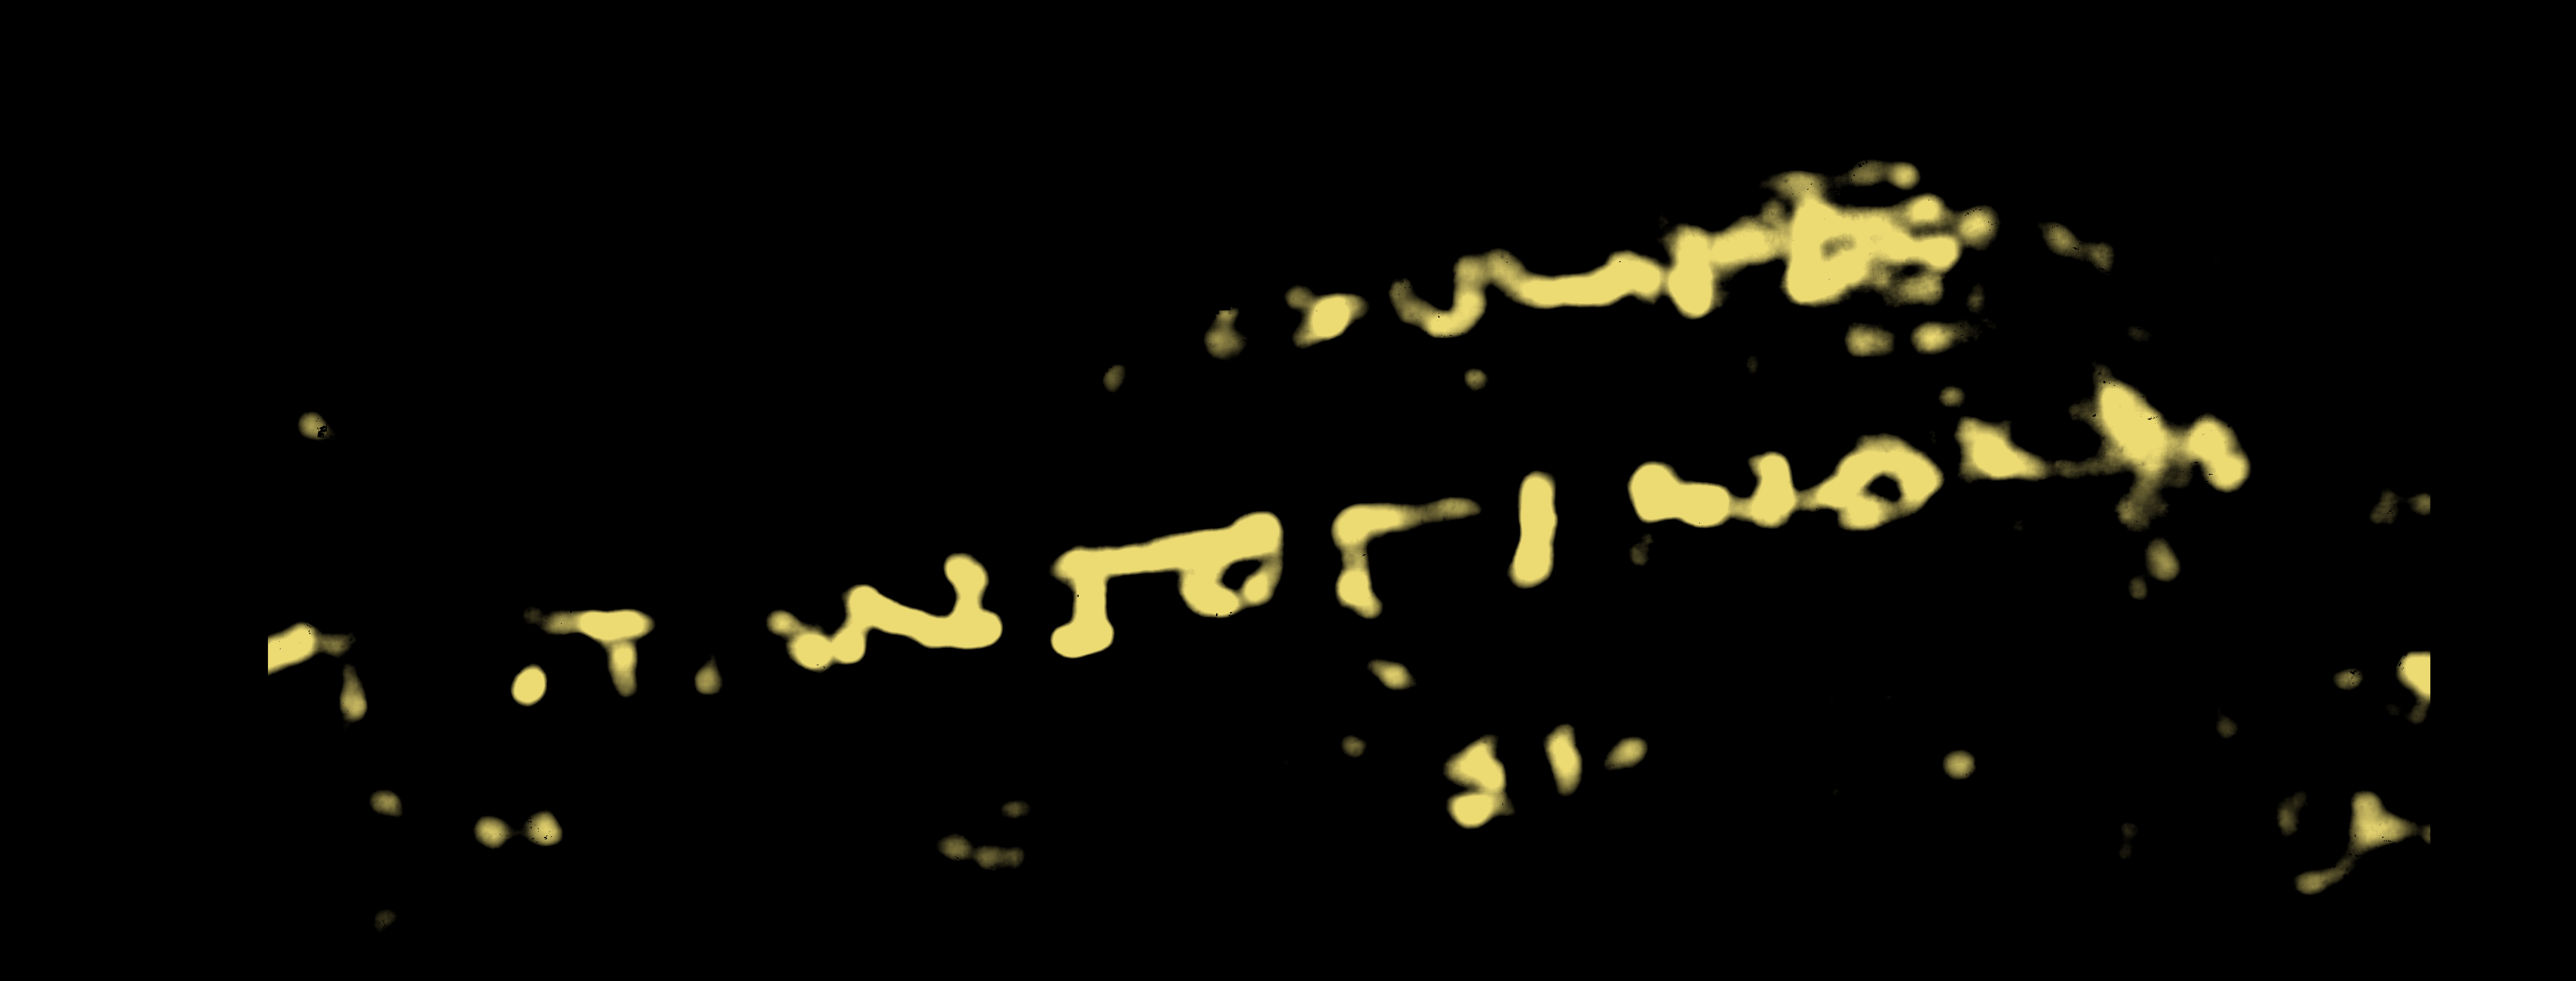
\includegraphics[width=0.29\textwidth]{../figures/m3/0343_1_reader-v3.png}
\hspace{3pt}
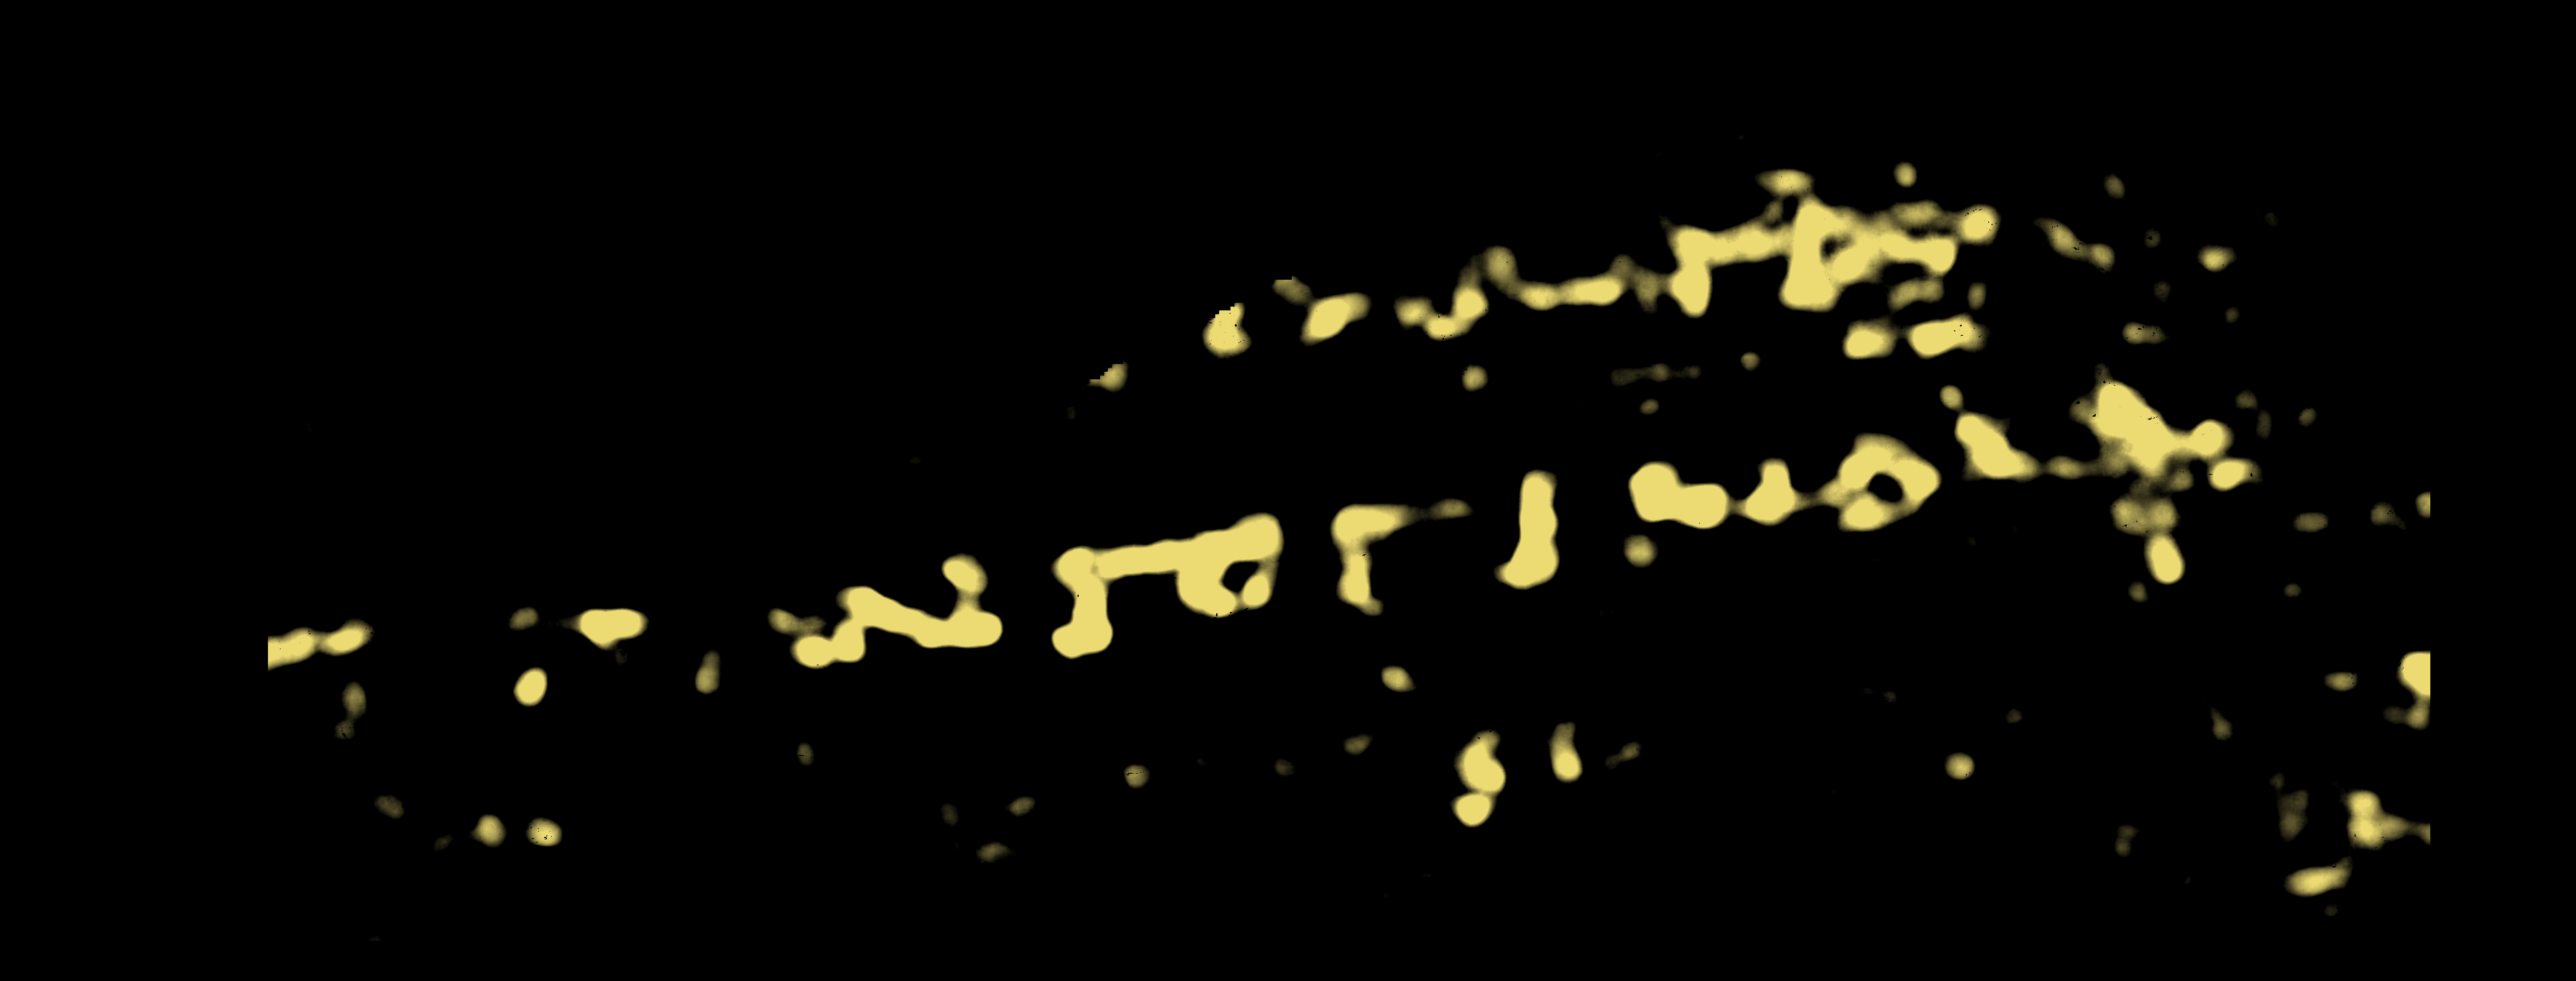
\includegraphics[width=0.29\textwidth]{../figures/m3/0343_2_m3.png}
\hspace{3pt}
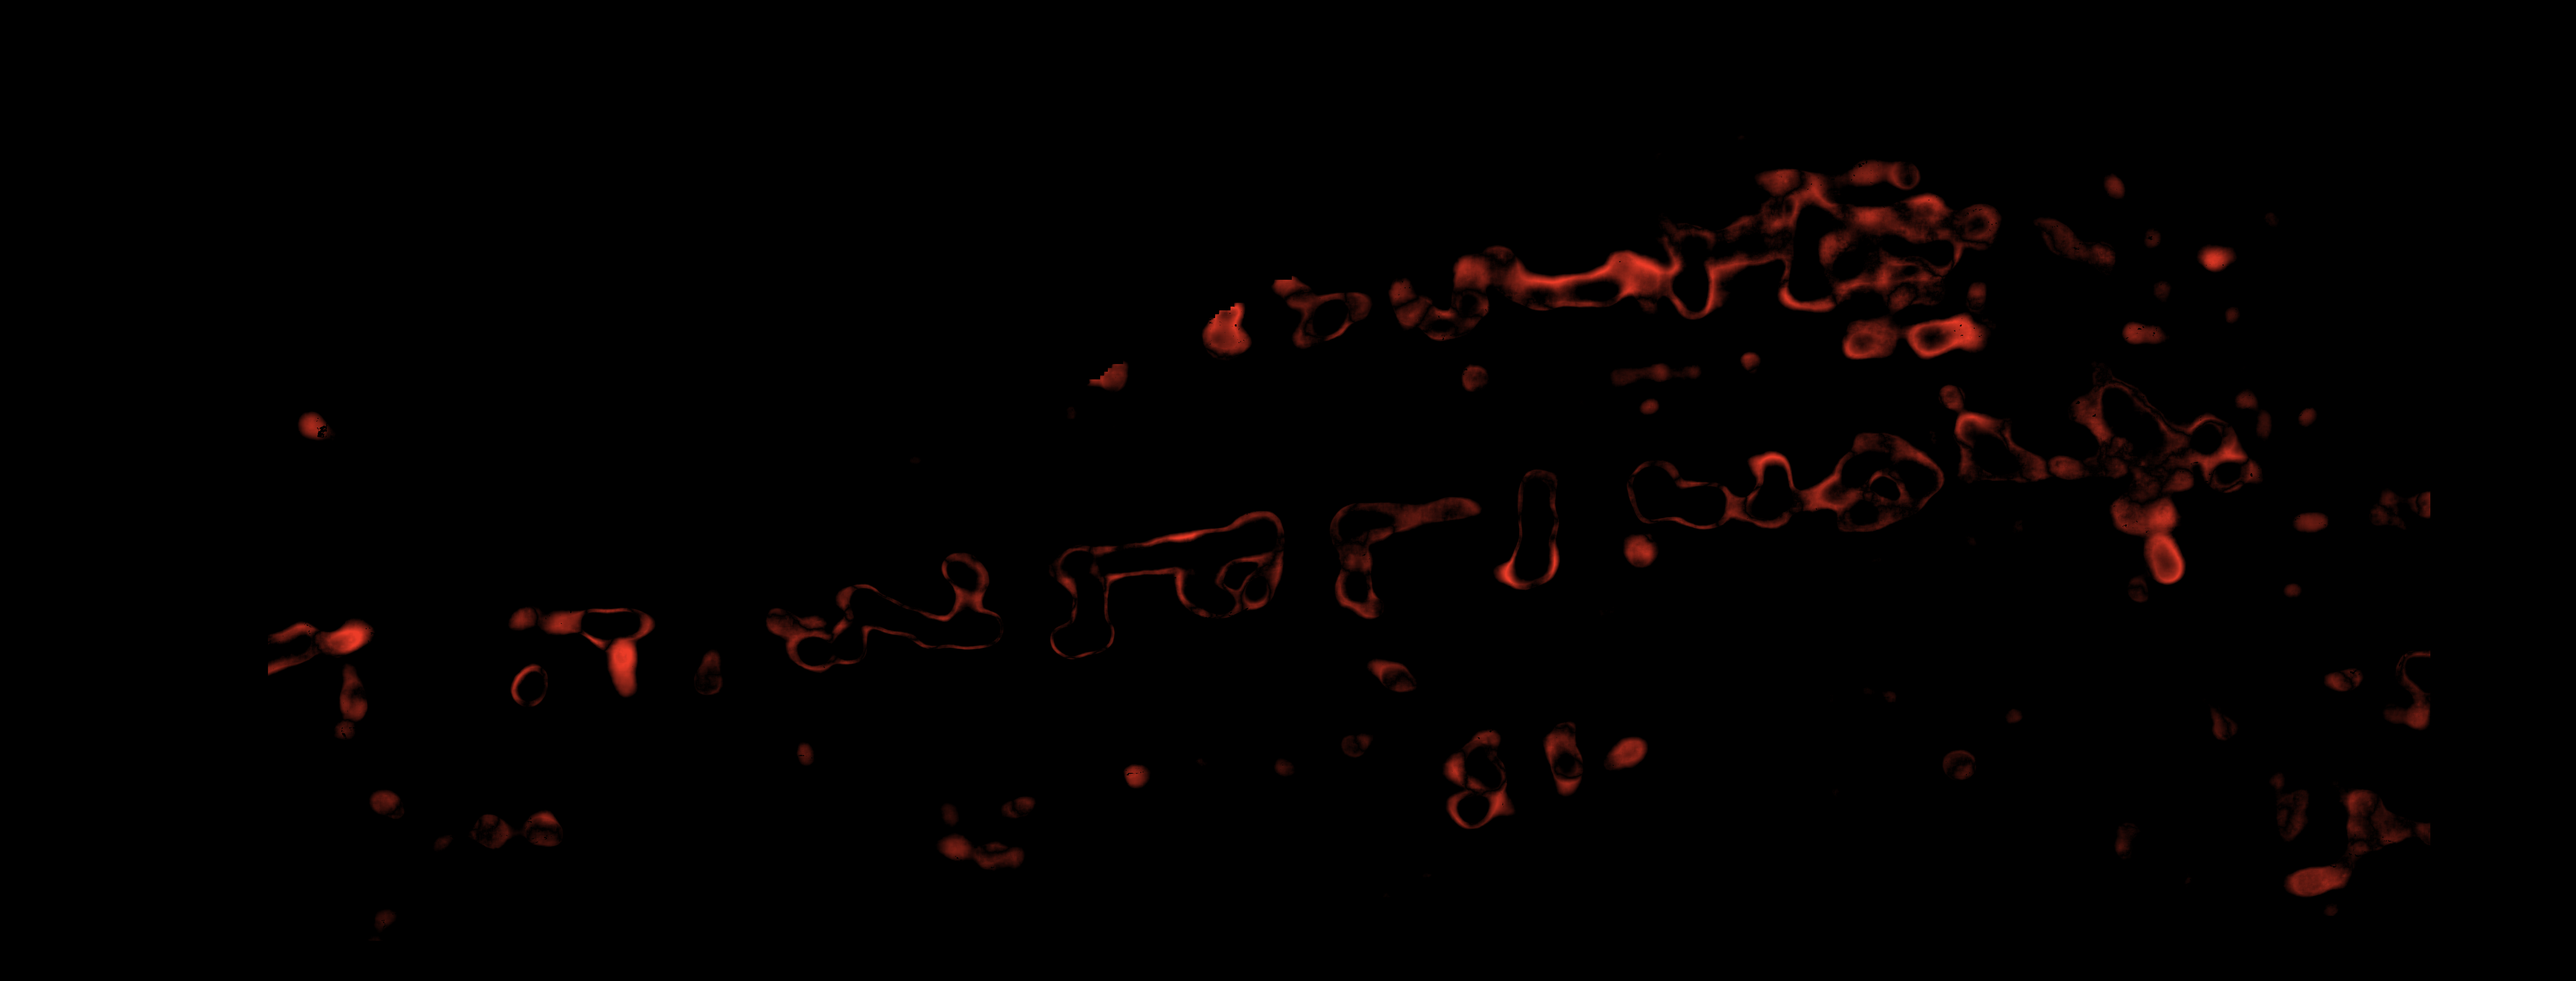
\includegraphics[width=0.29\textwidth]{../figures/m3/0343_3_difference.png}
\caption{Control unit 0343. Left, Reader v3 (AUC 0.9078); centre, \MtName{} (AUC 0.8911); right, the red difference between the two maps. Each map is stretched between its own percentiles, the panels are shown at the full resolution of the file.}\label{fig:m3-0343}
\end{figure*}

\begin{figure*}[!tp]
\centering
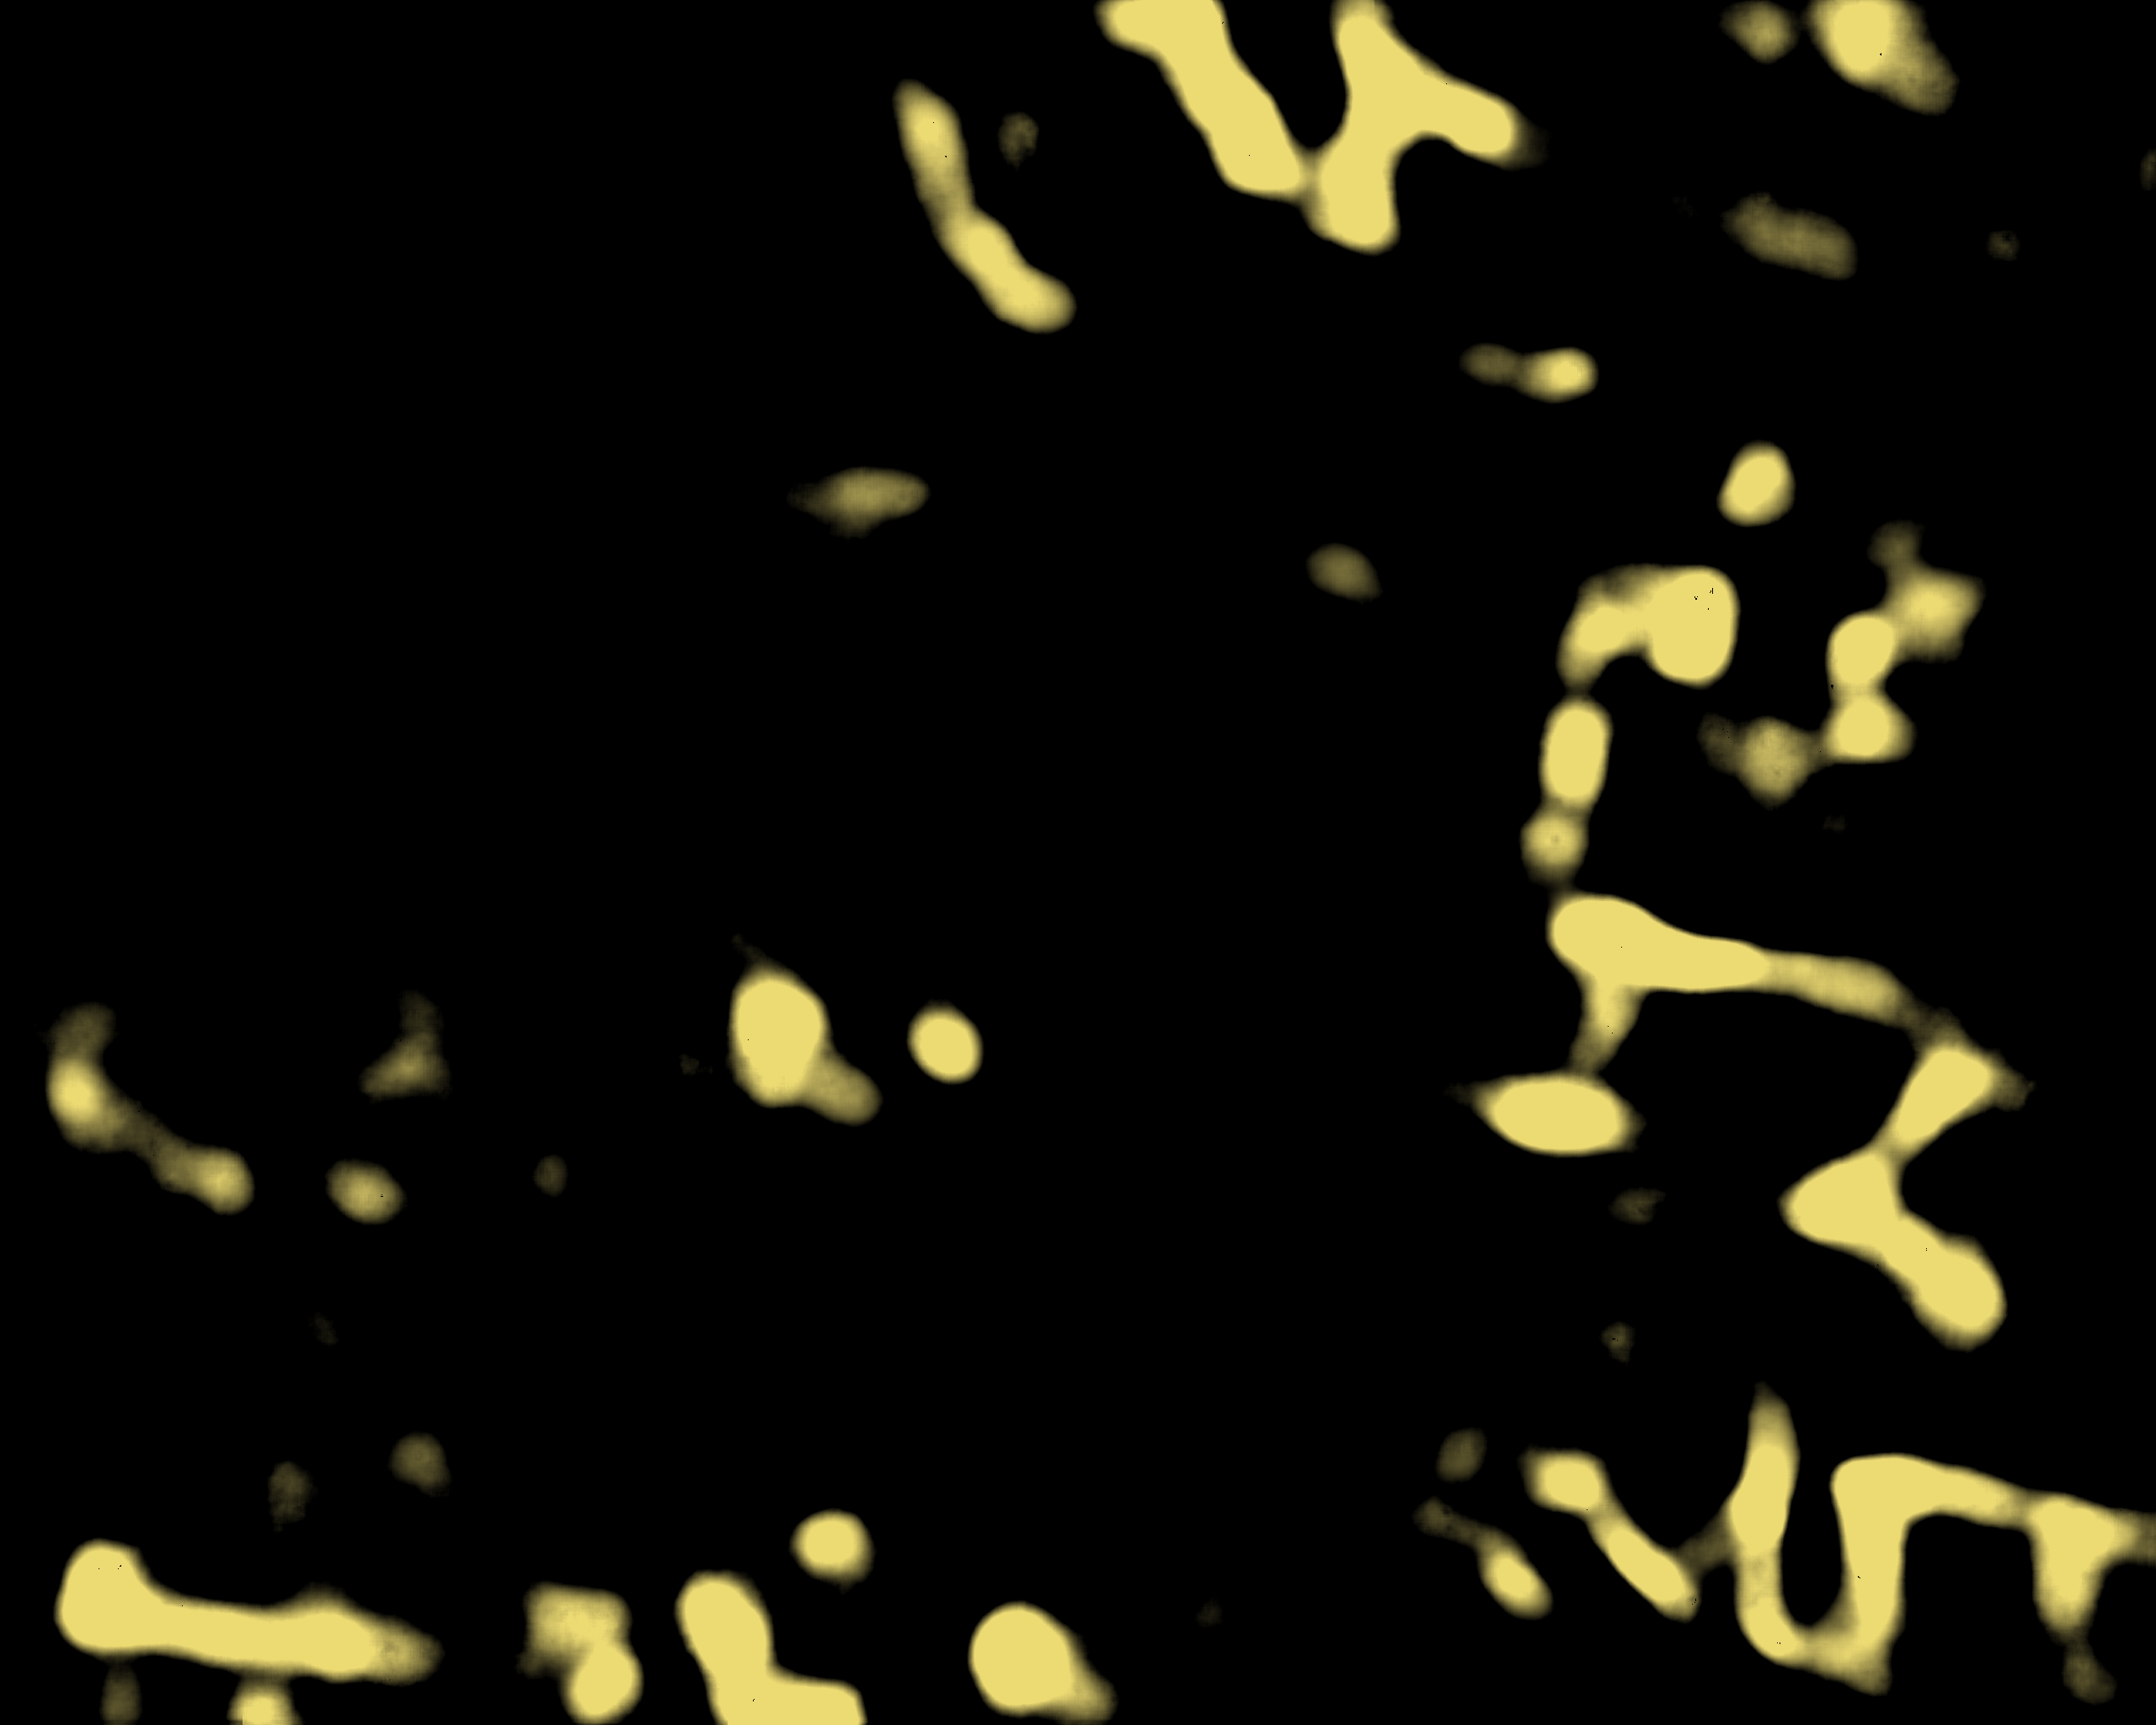
\includegraphics[width=0.29\textwidth]{../figures/m3/ag1_1_reader-v3.png}
\hspace{3pt}
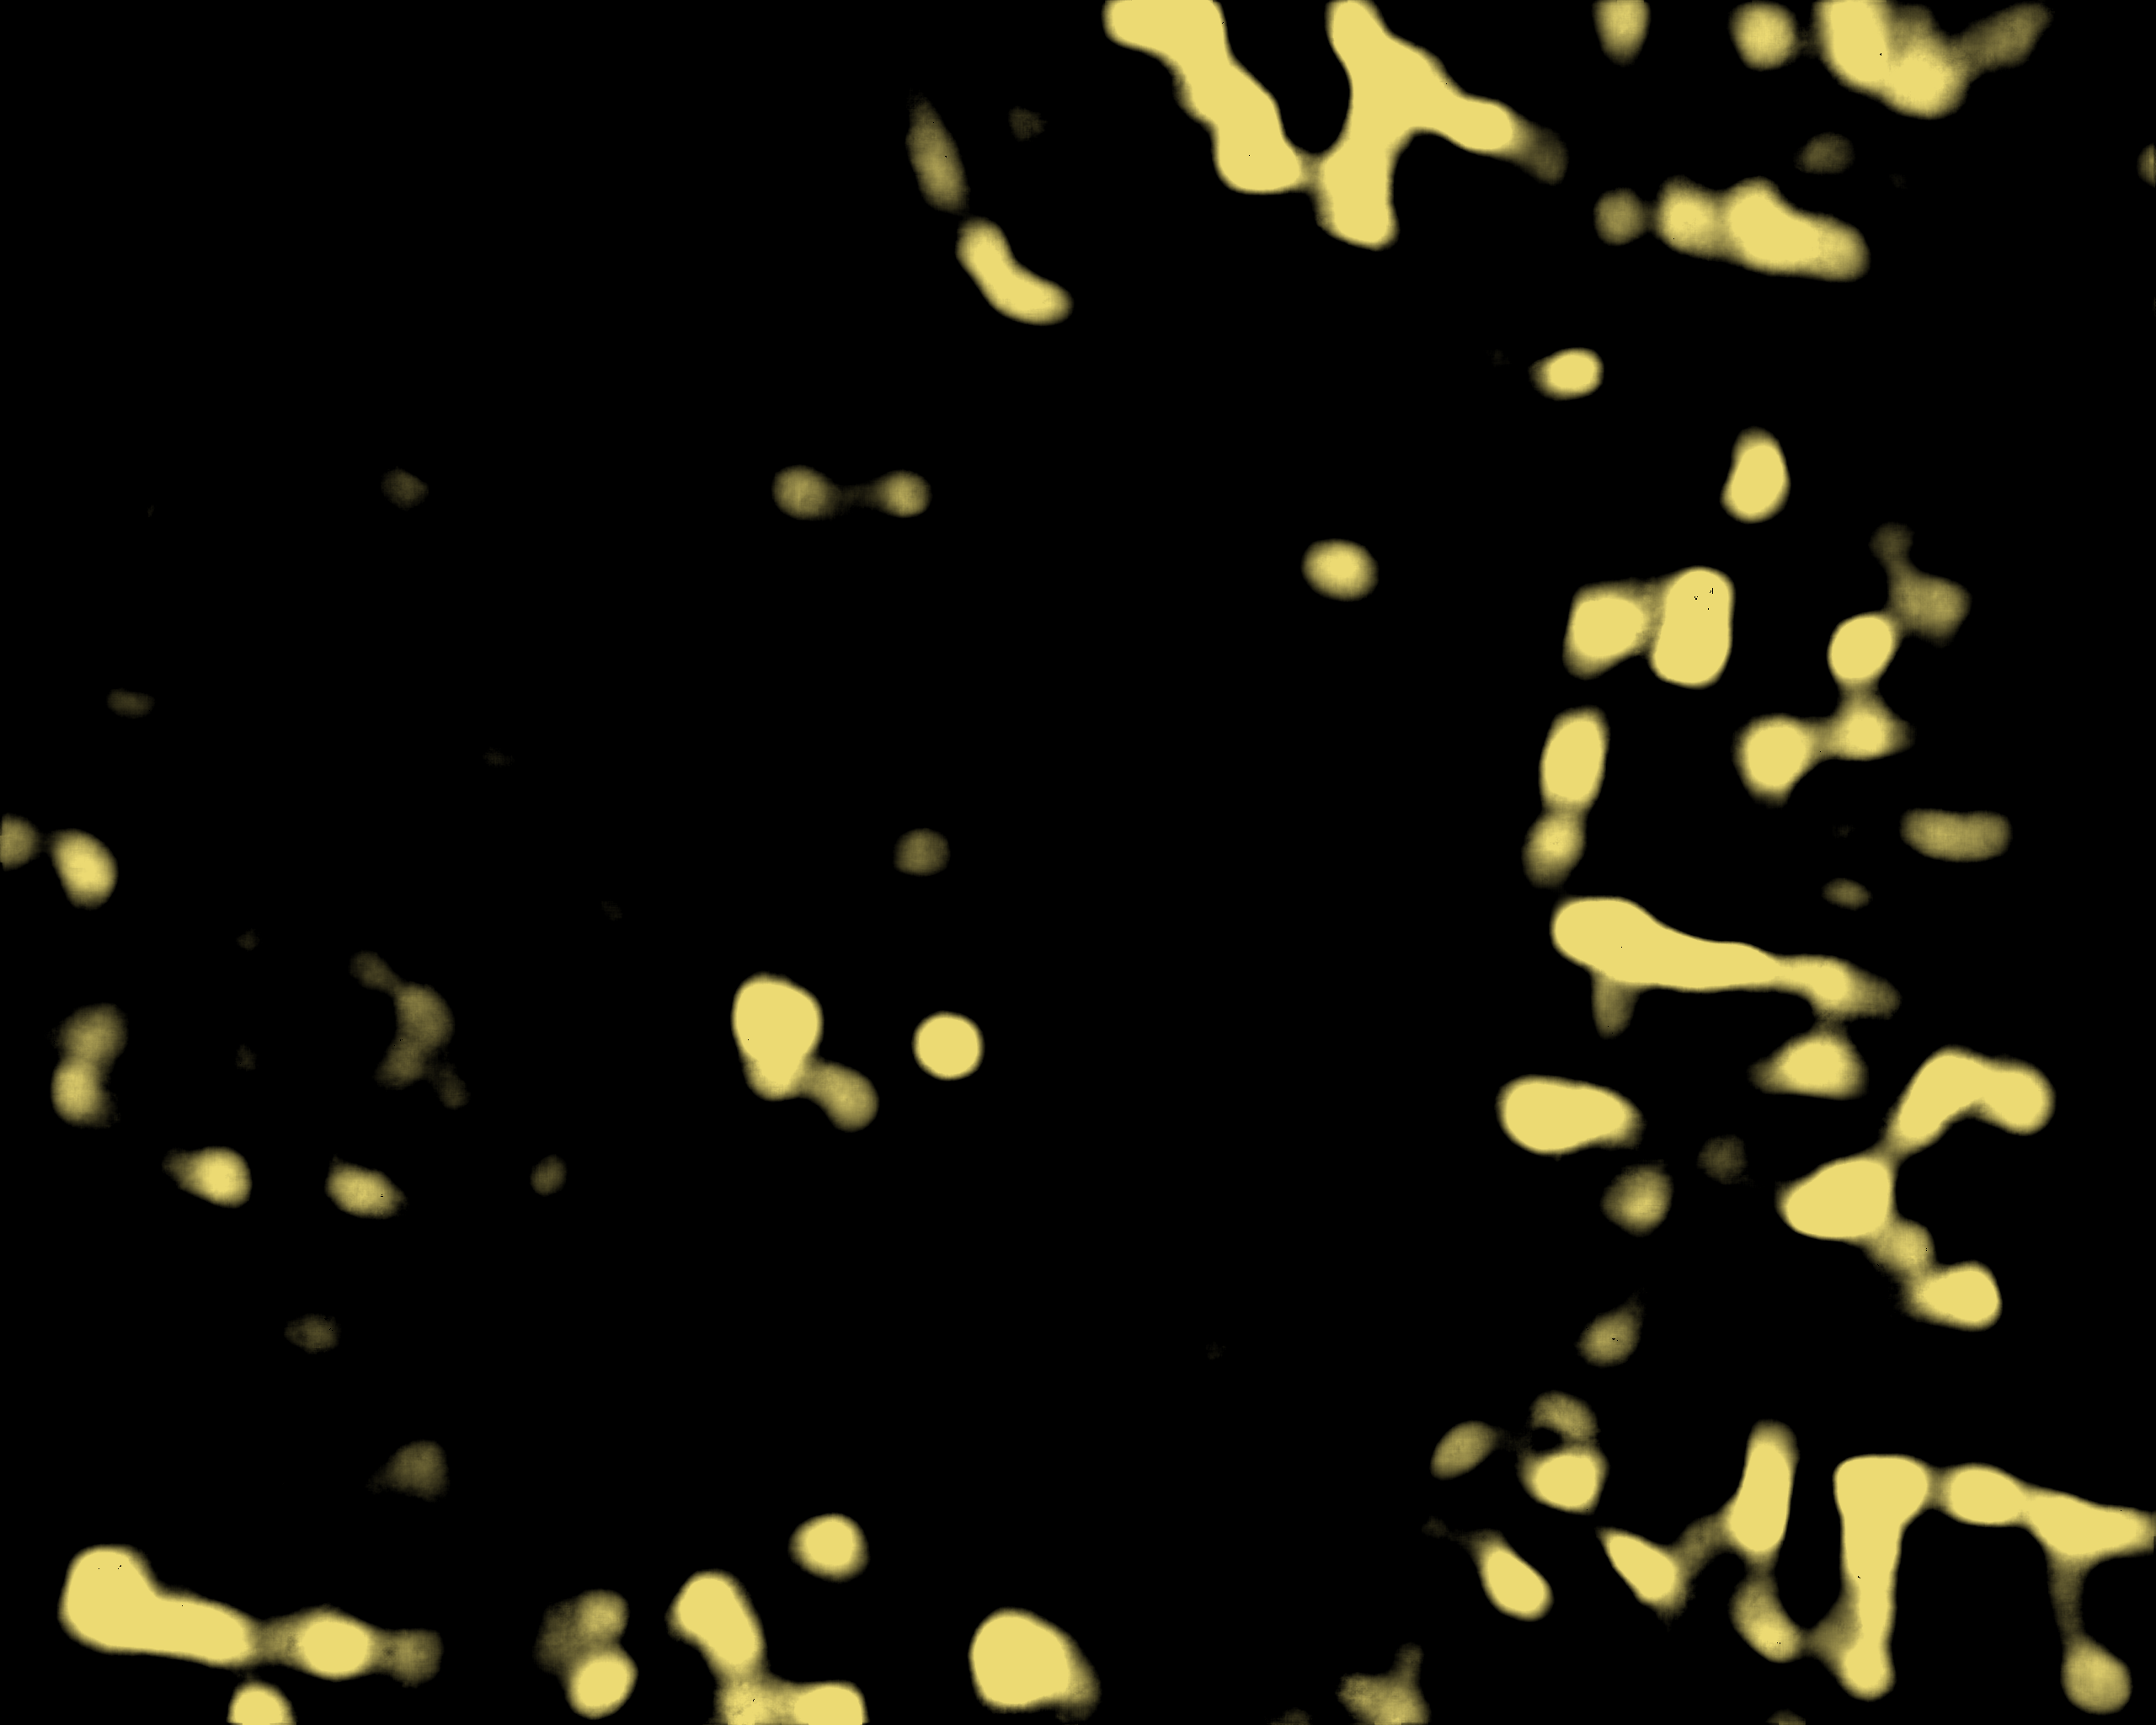
\includegraphics[width=0.29\textwidth]{../figures/m3/ag1_2_m3.png}
\hspace{3pt}
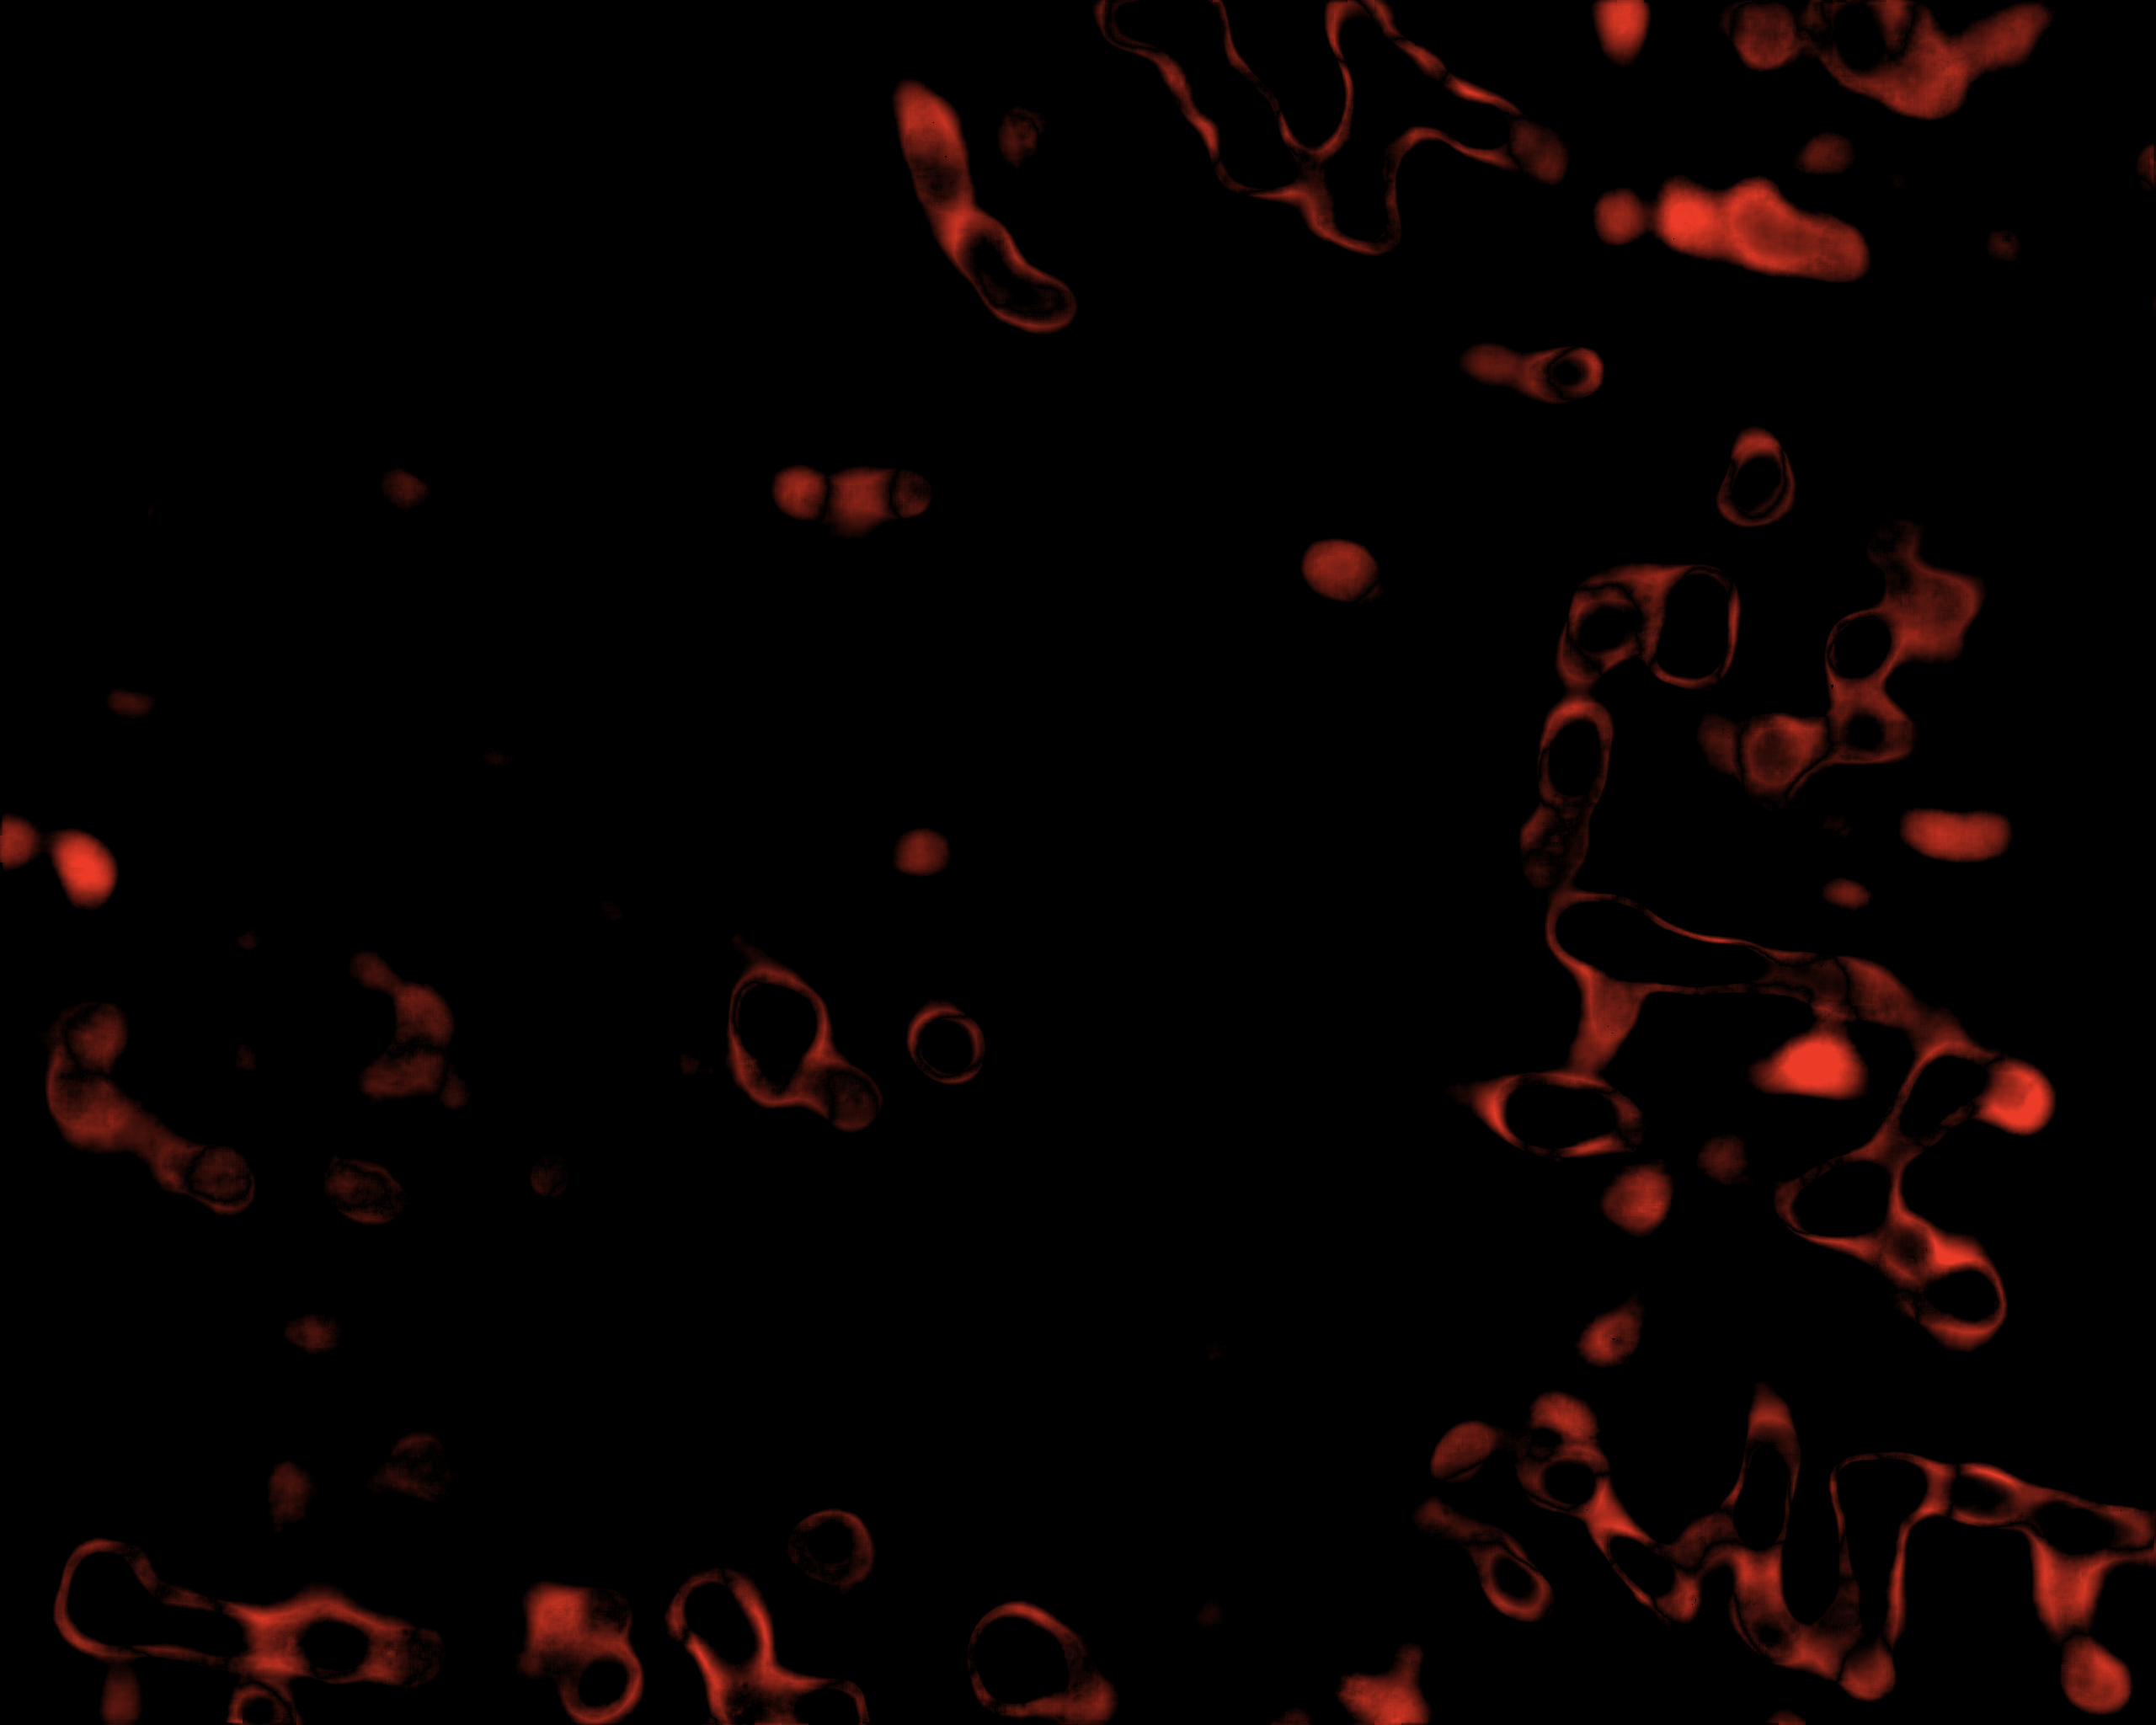
\includegraphics[width=0.29\textwidth]{../figures/m3/ag1_3_difference.png}
\caption{Control unit 0841 ag1. Left, Reader v3 (AUC 0.8513); centre, \MtName{} (AUC 0.8532); right, the red difference between the two maps. Each map is stretched between its own percentiles, the panels are shown at the full resolution of the file.}\label{fig:m3-ag1}
\end{figure*}

\begin{figure*}[!tp]
\centering
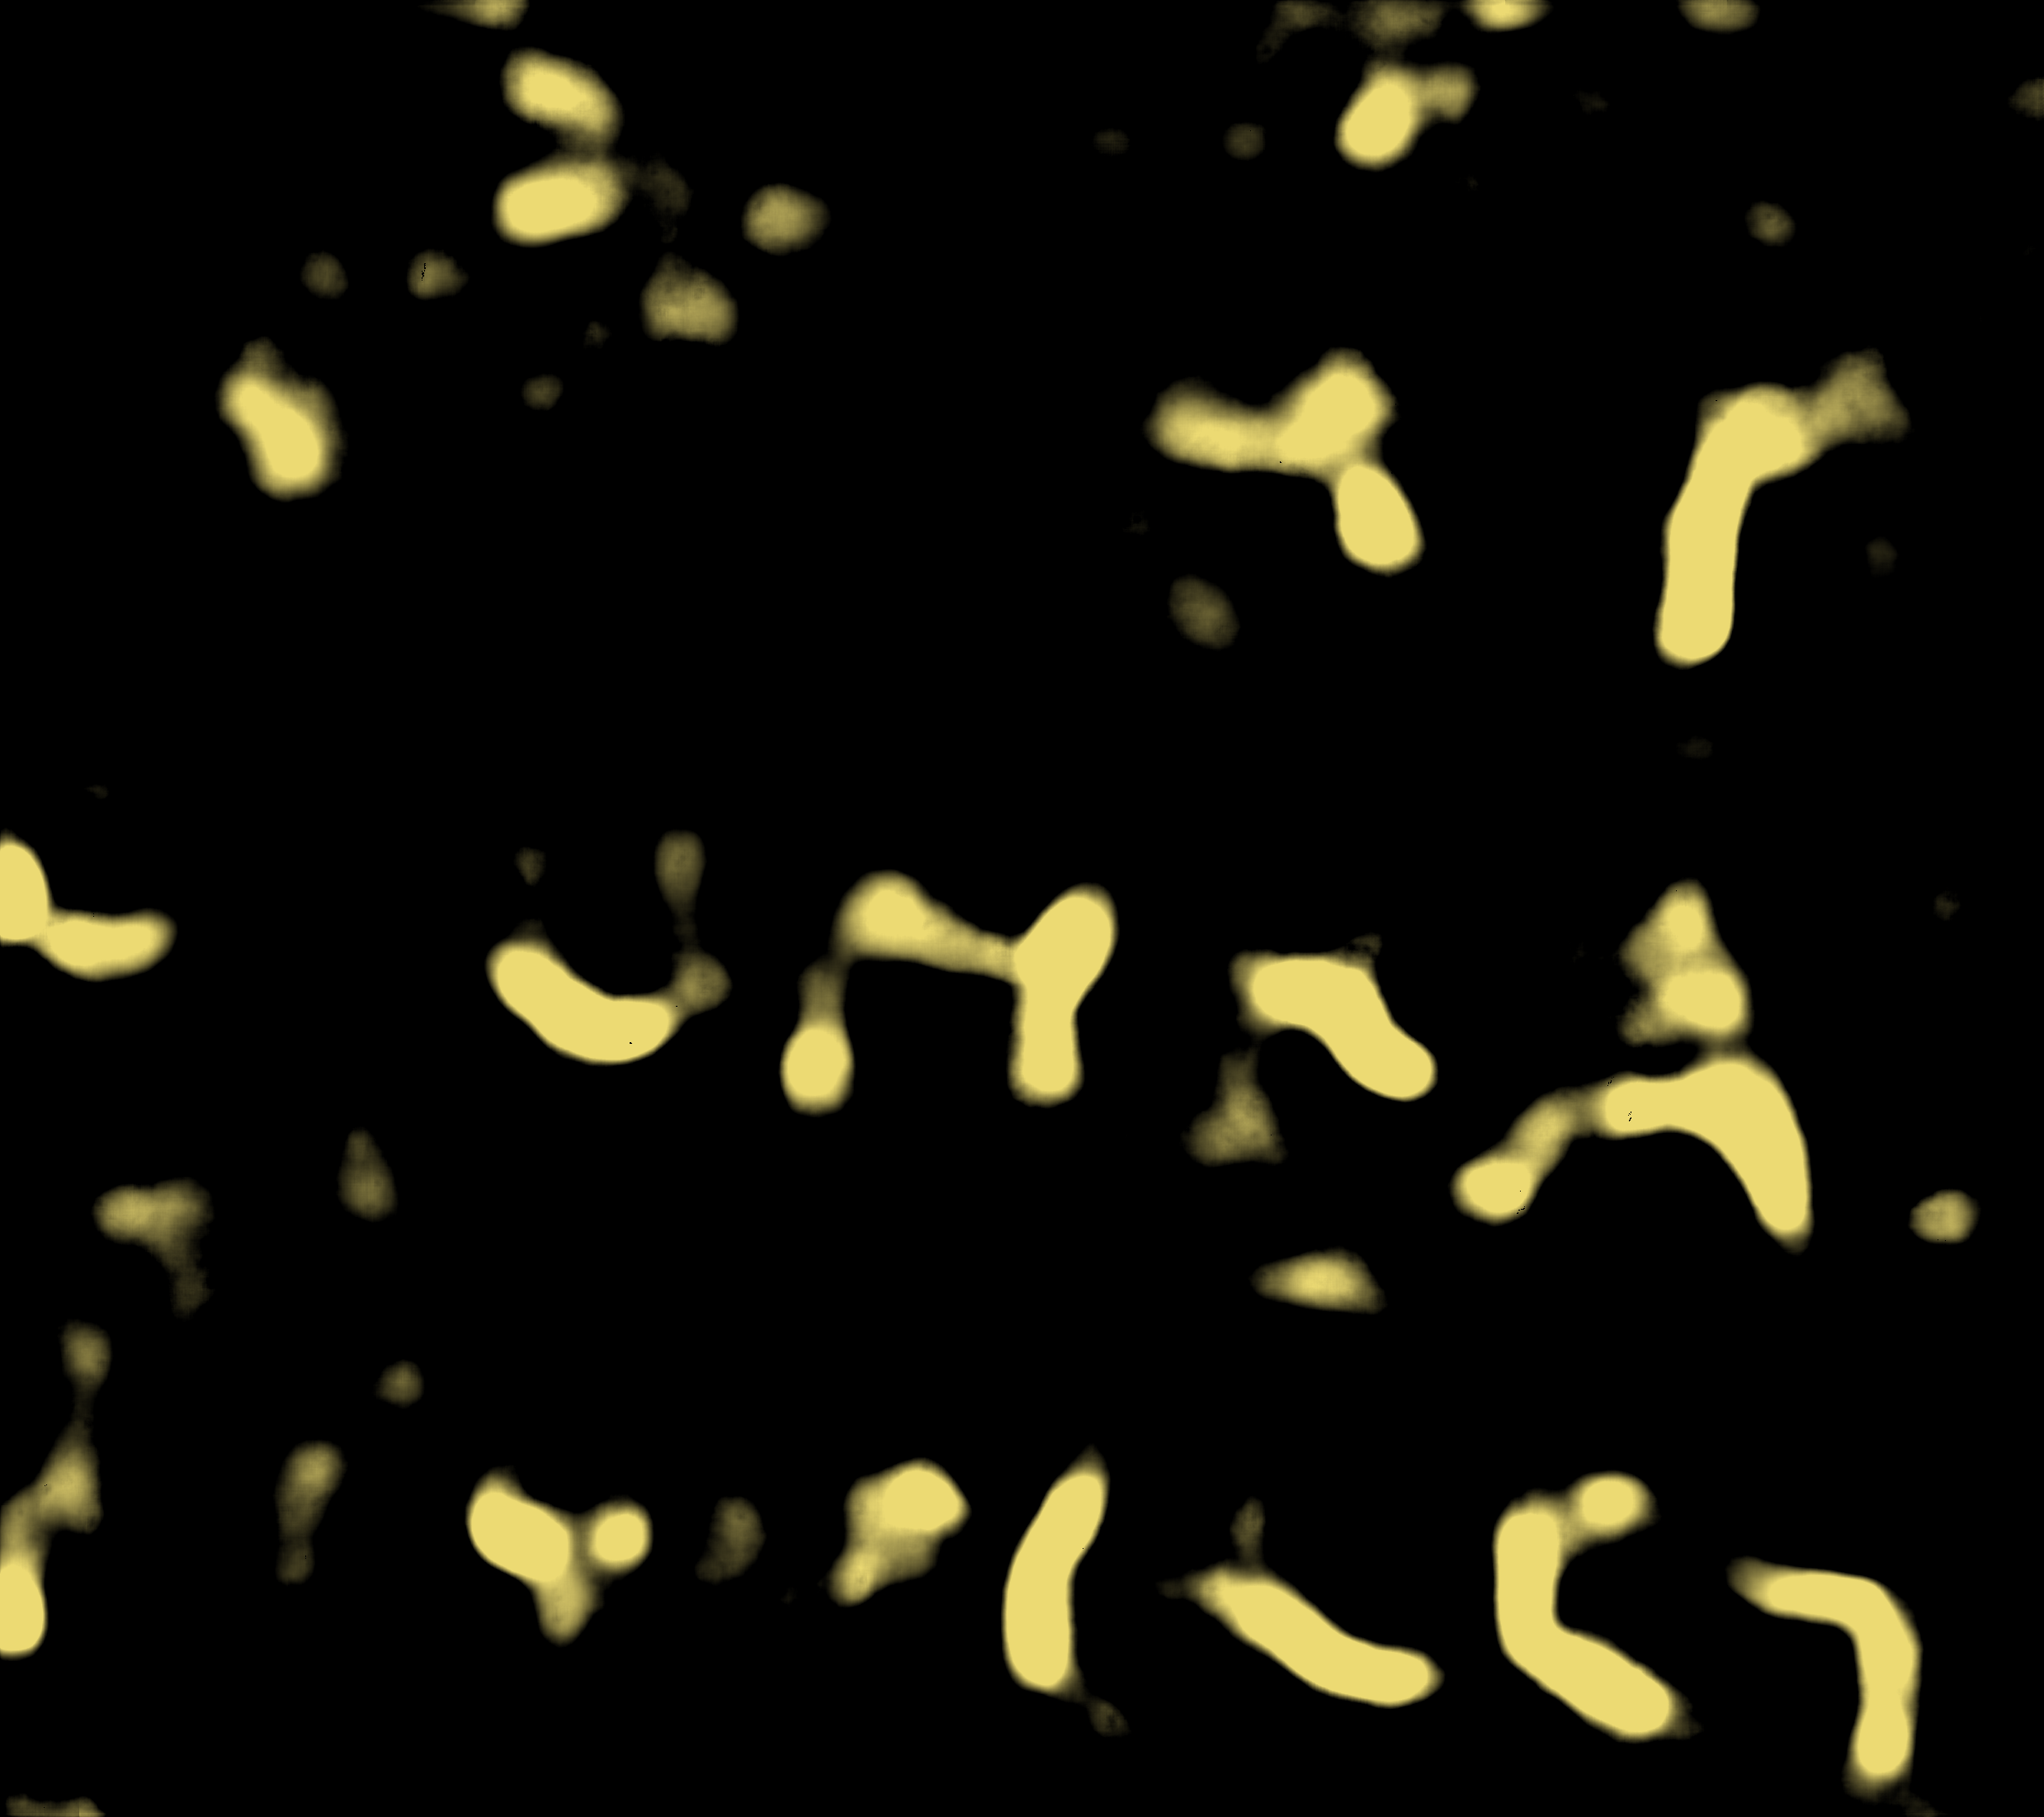
\includegraphics[width=0.29\textwidth]{../figures/m3/ag2_1_reader-v3.png}
\hspace{3pt}
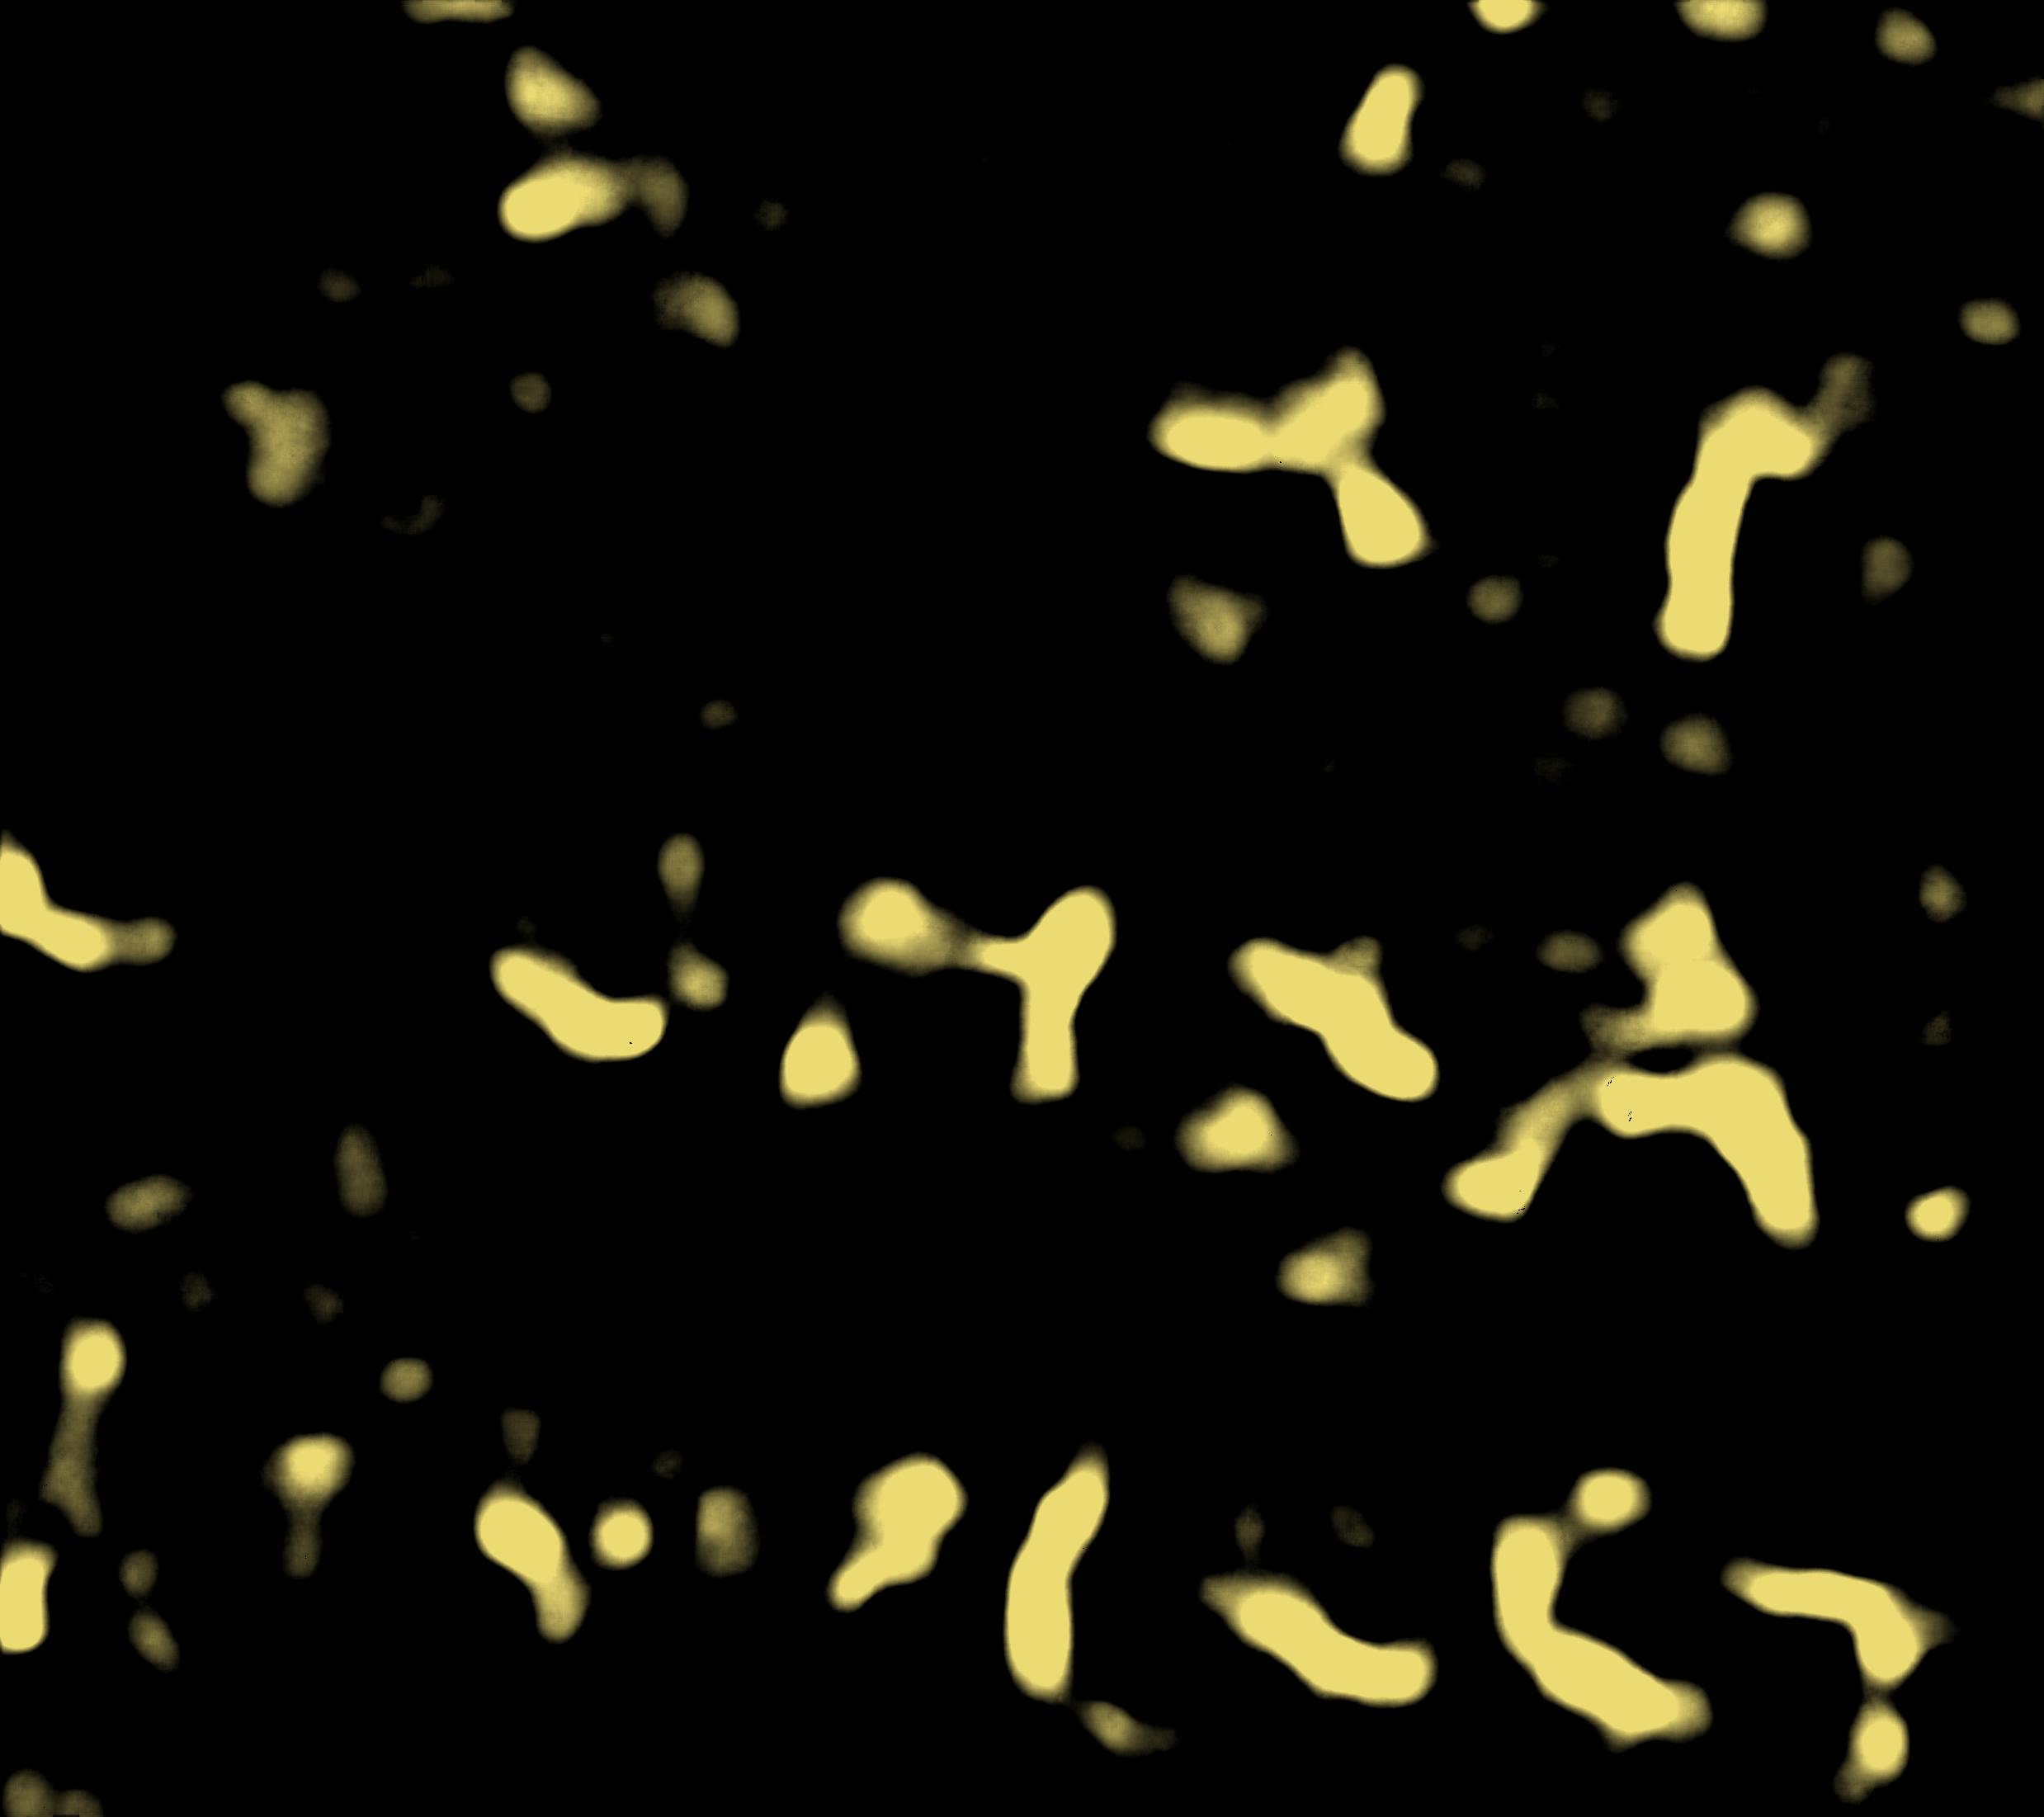
\includegraphics[width=0.29\textwidth]{../figures/m3/ag2_2_m3.png}
\hspace{3pt}
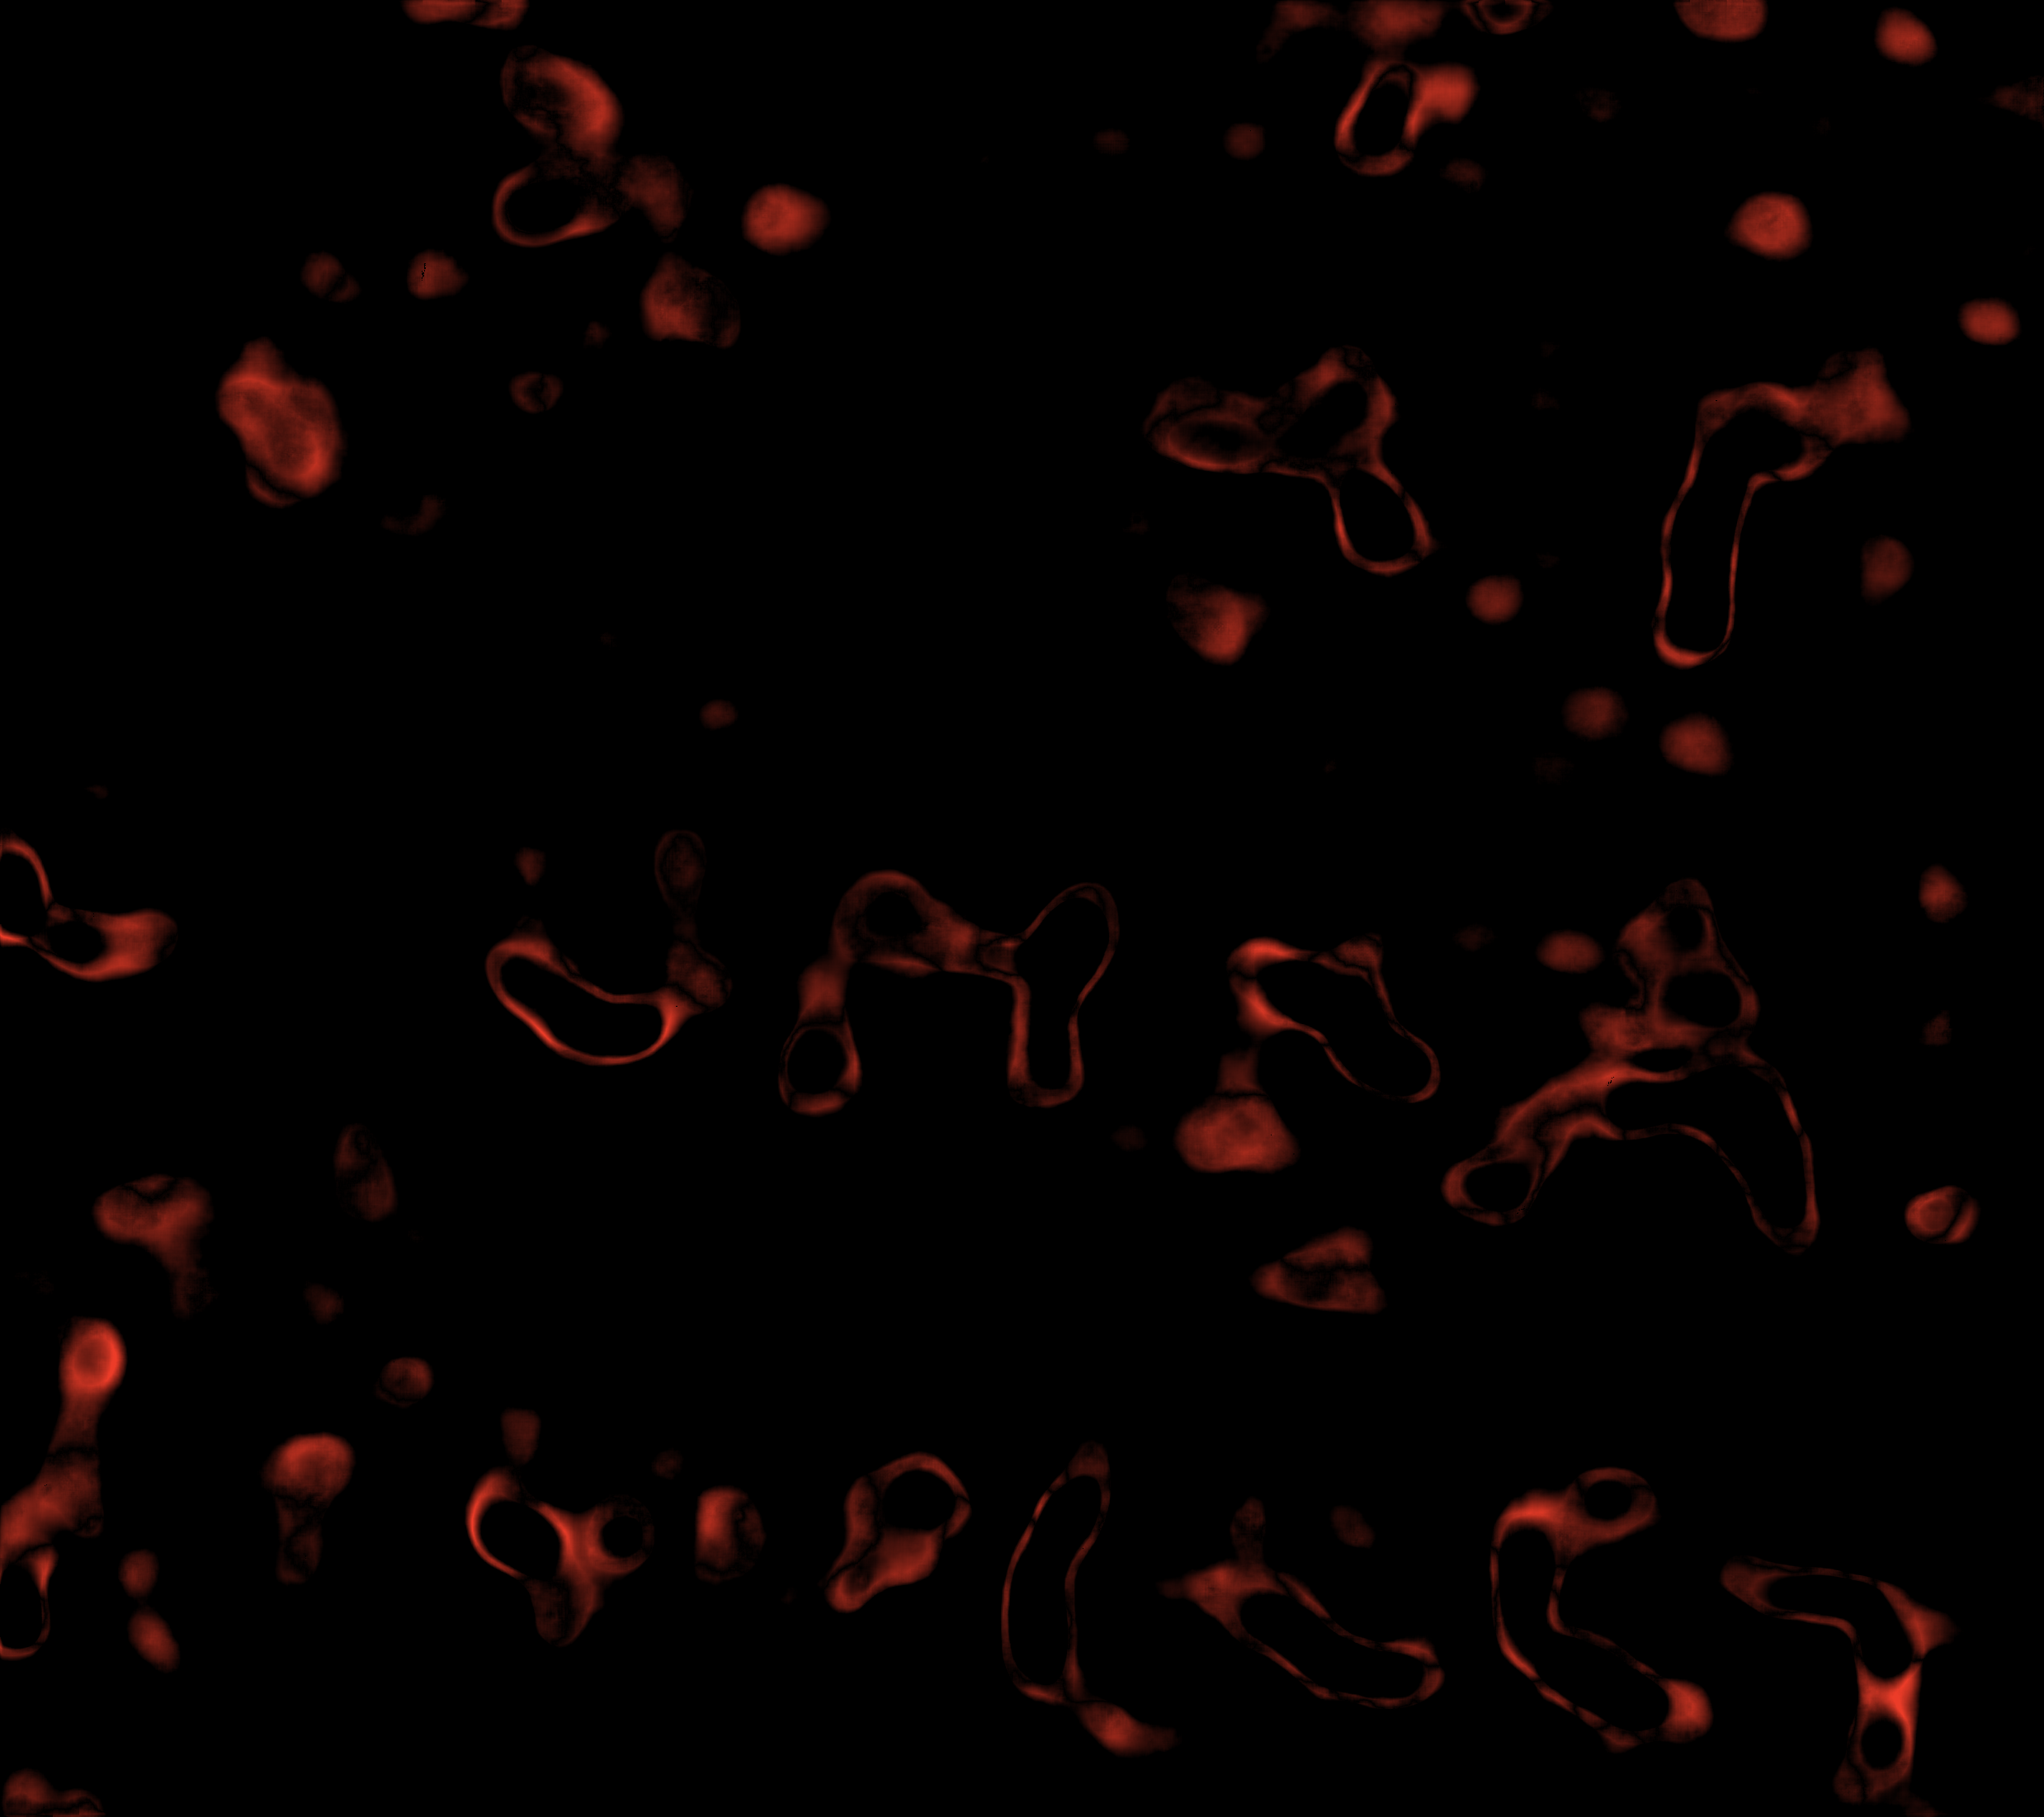
\includegraphics[width=0.29\textwidth]{../figures/m3/ag2_3_difference.png}
\caption{Control unit 0841 ag2. Left, Reader v3 (AUC 0.8297); centre, \MtName{} (AUC 0.8390); right, the red difference between the two maps. Each map is stretched between its own percentiles, the panels are shown at the full resolution of the file.}\label{fig:m3-ag2}
\end{figure*}

\begin{figure*}[!tp]
\centering
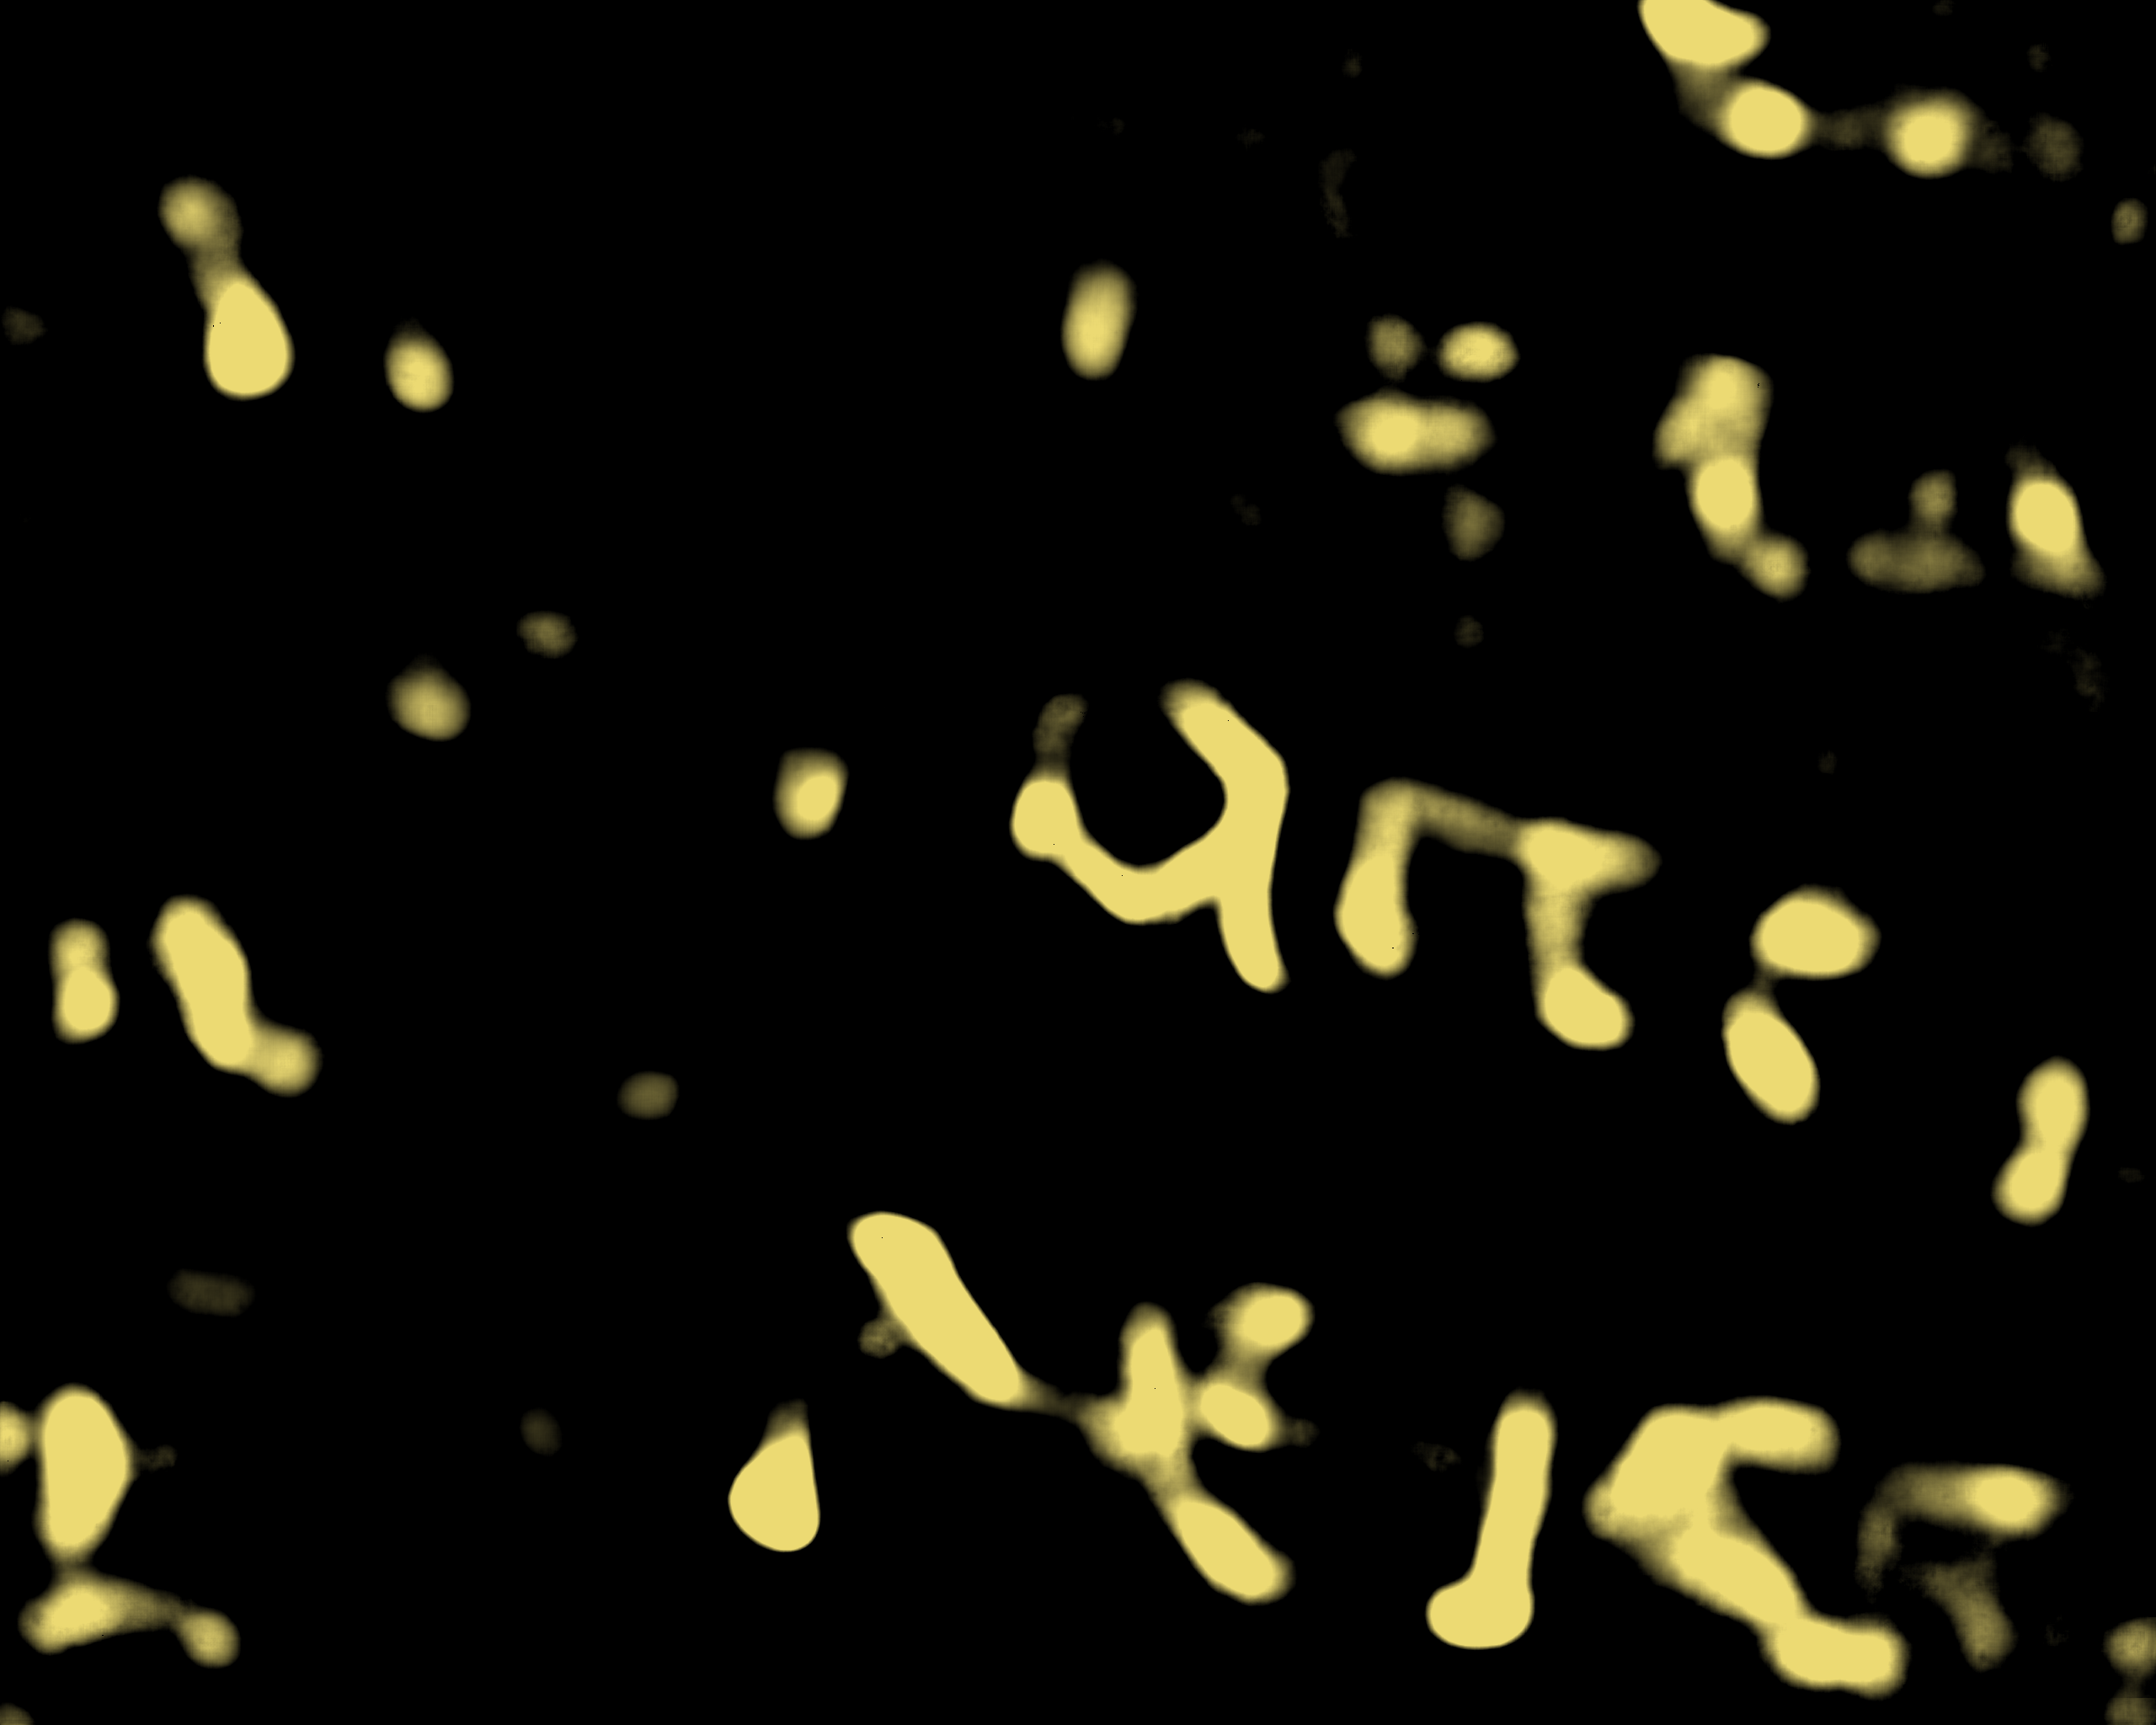
\includegraphics[width=0.29\textwidth]{../figures/m3/w00_1_reader-v3.png}
\hspace{3pt}
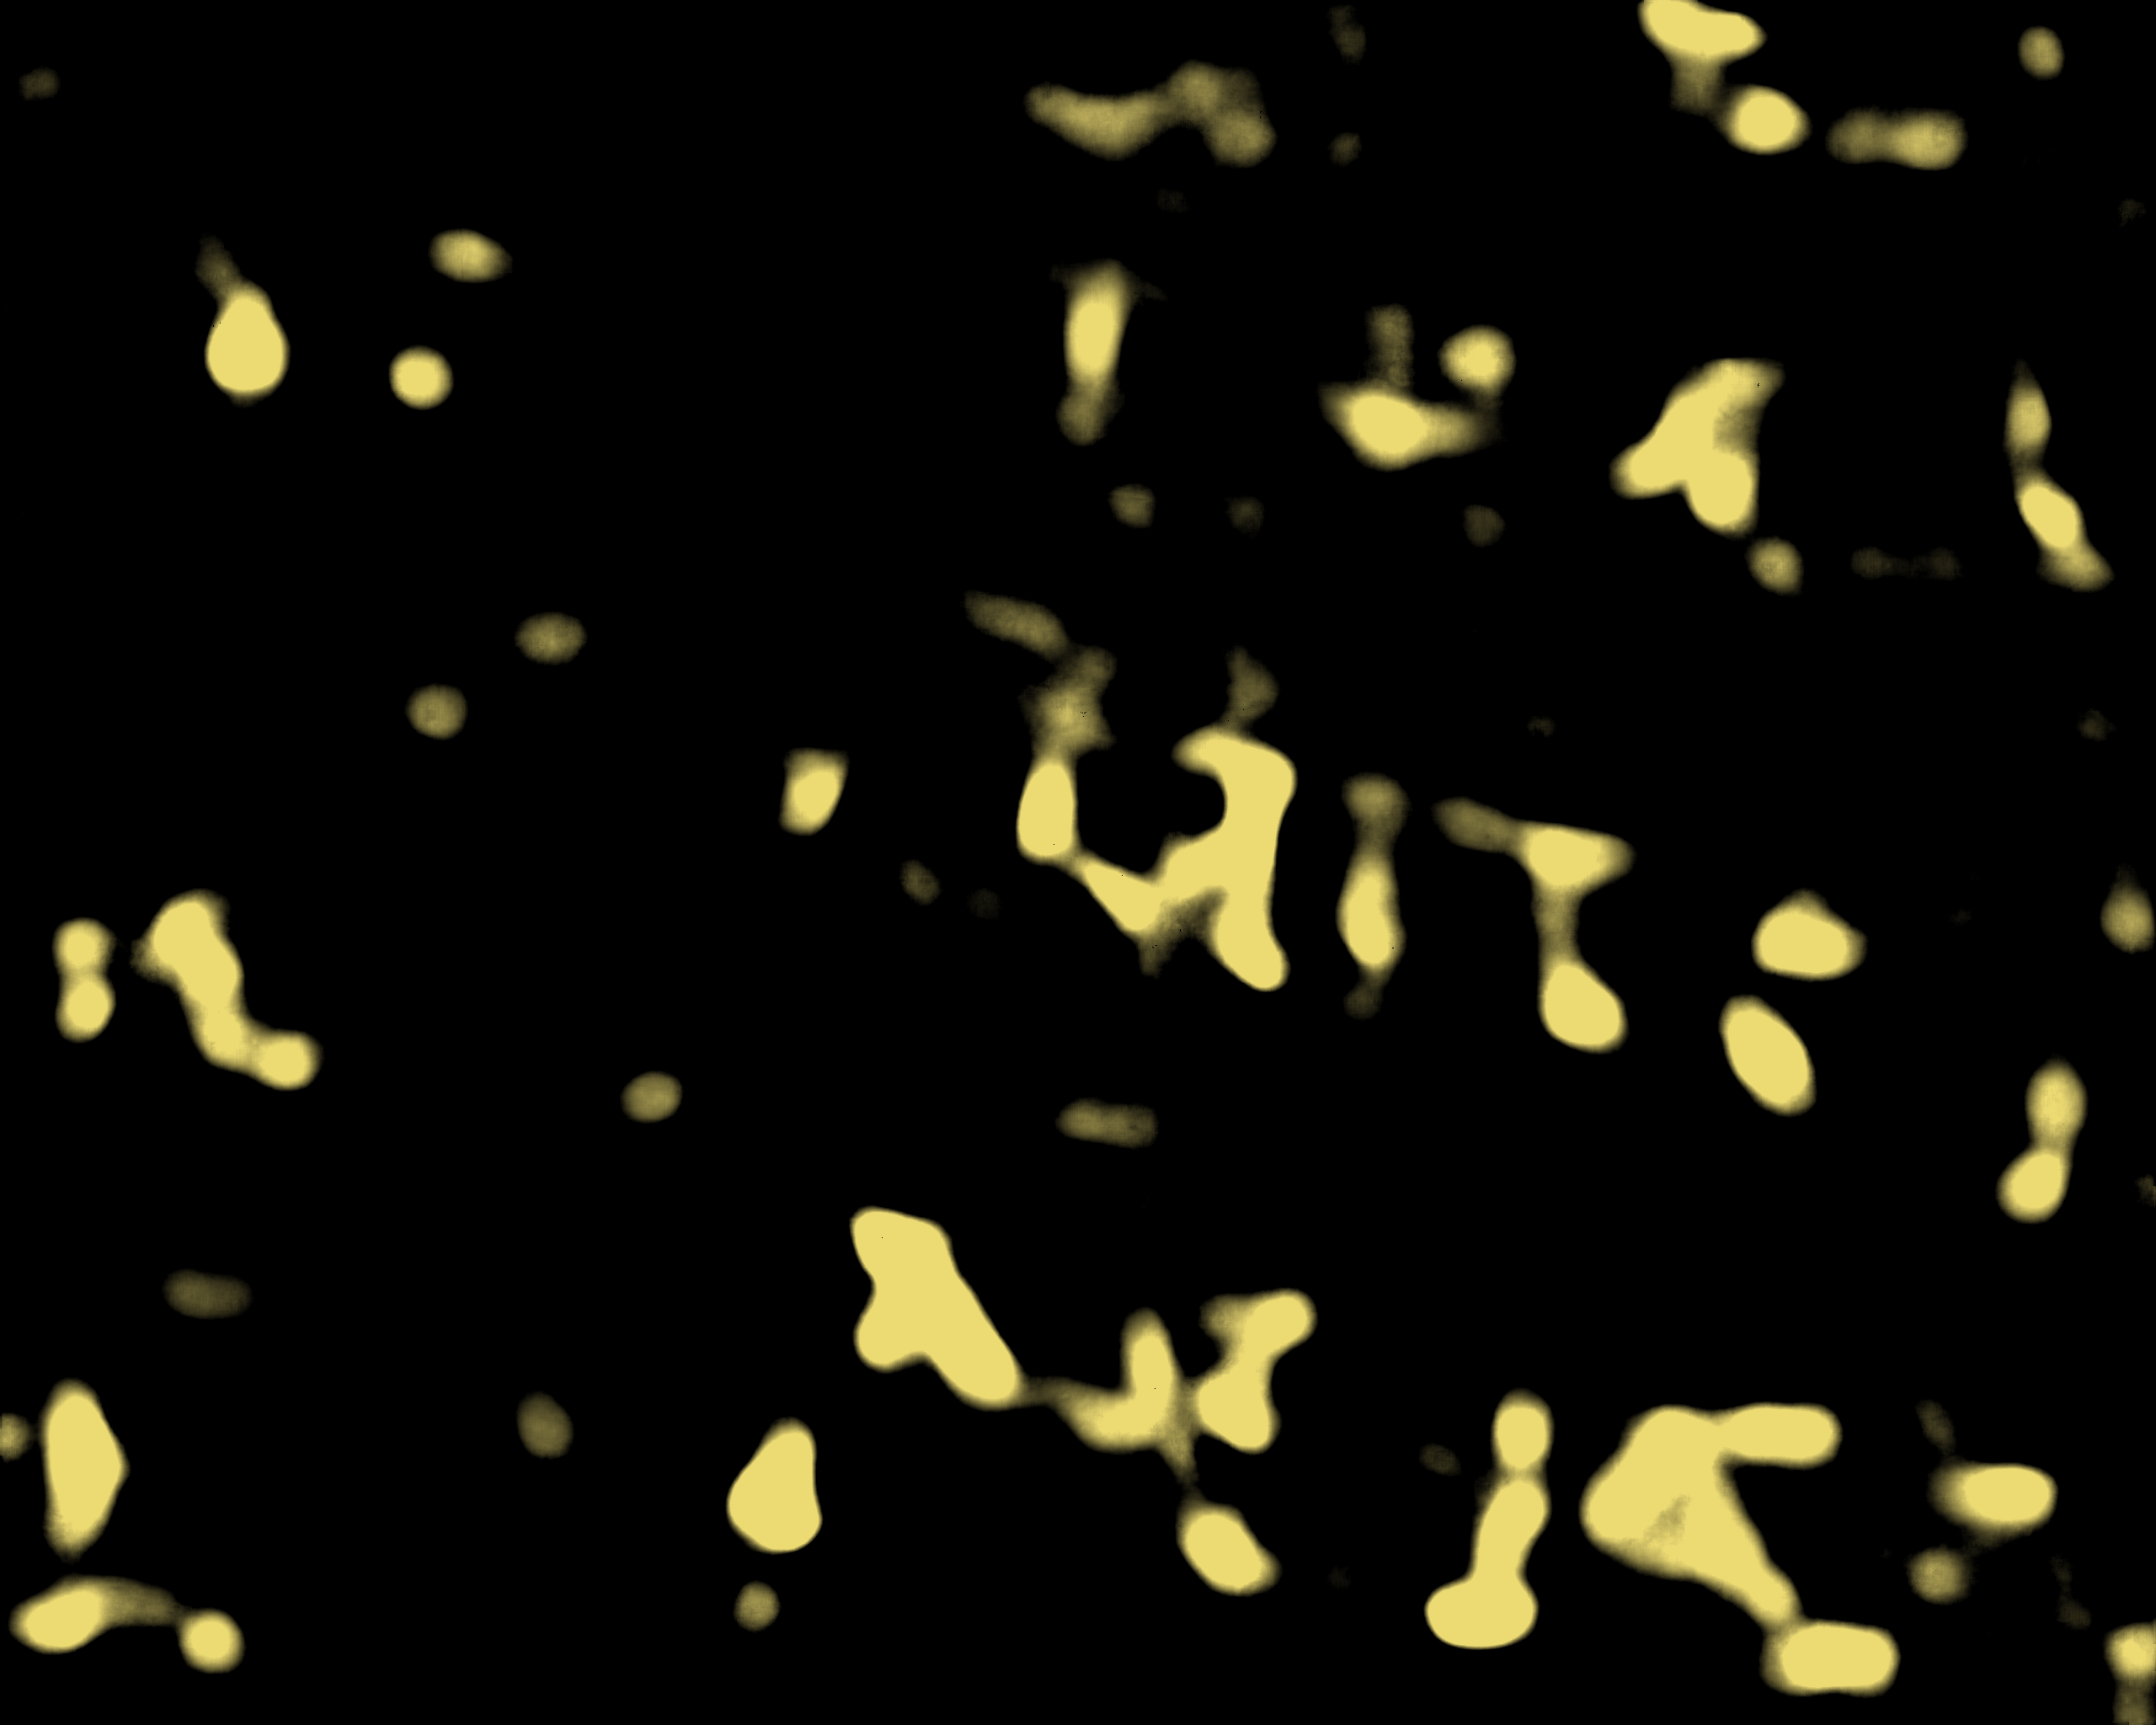
\includegraphics[width=0.29\textwidth]{../figures/m3/w00_2_m3.png}
\hspace{3pt}
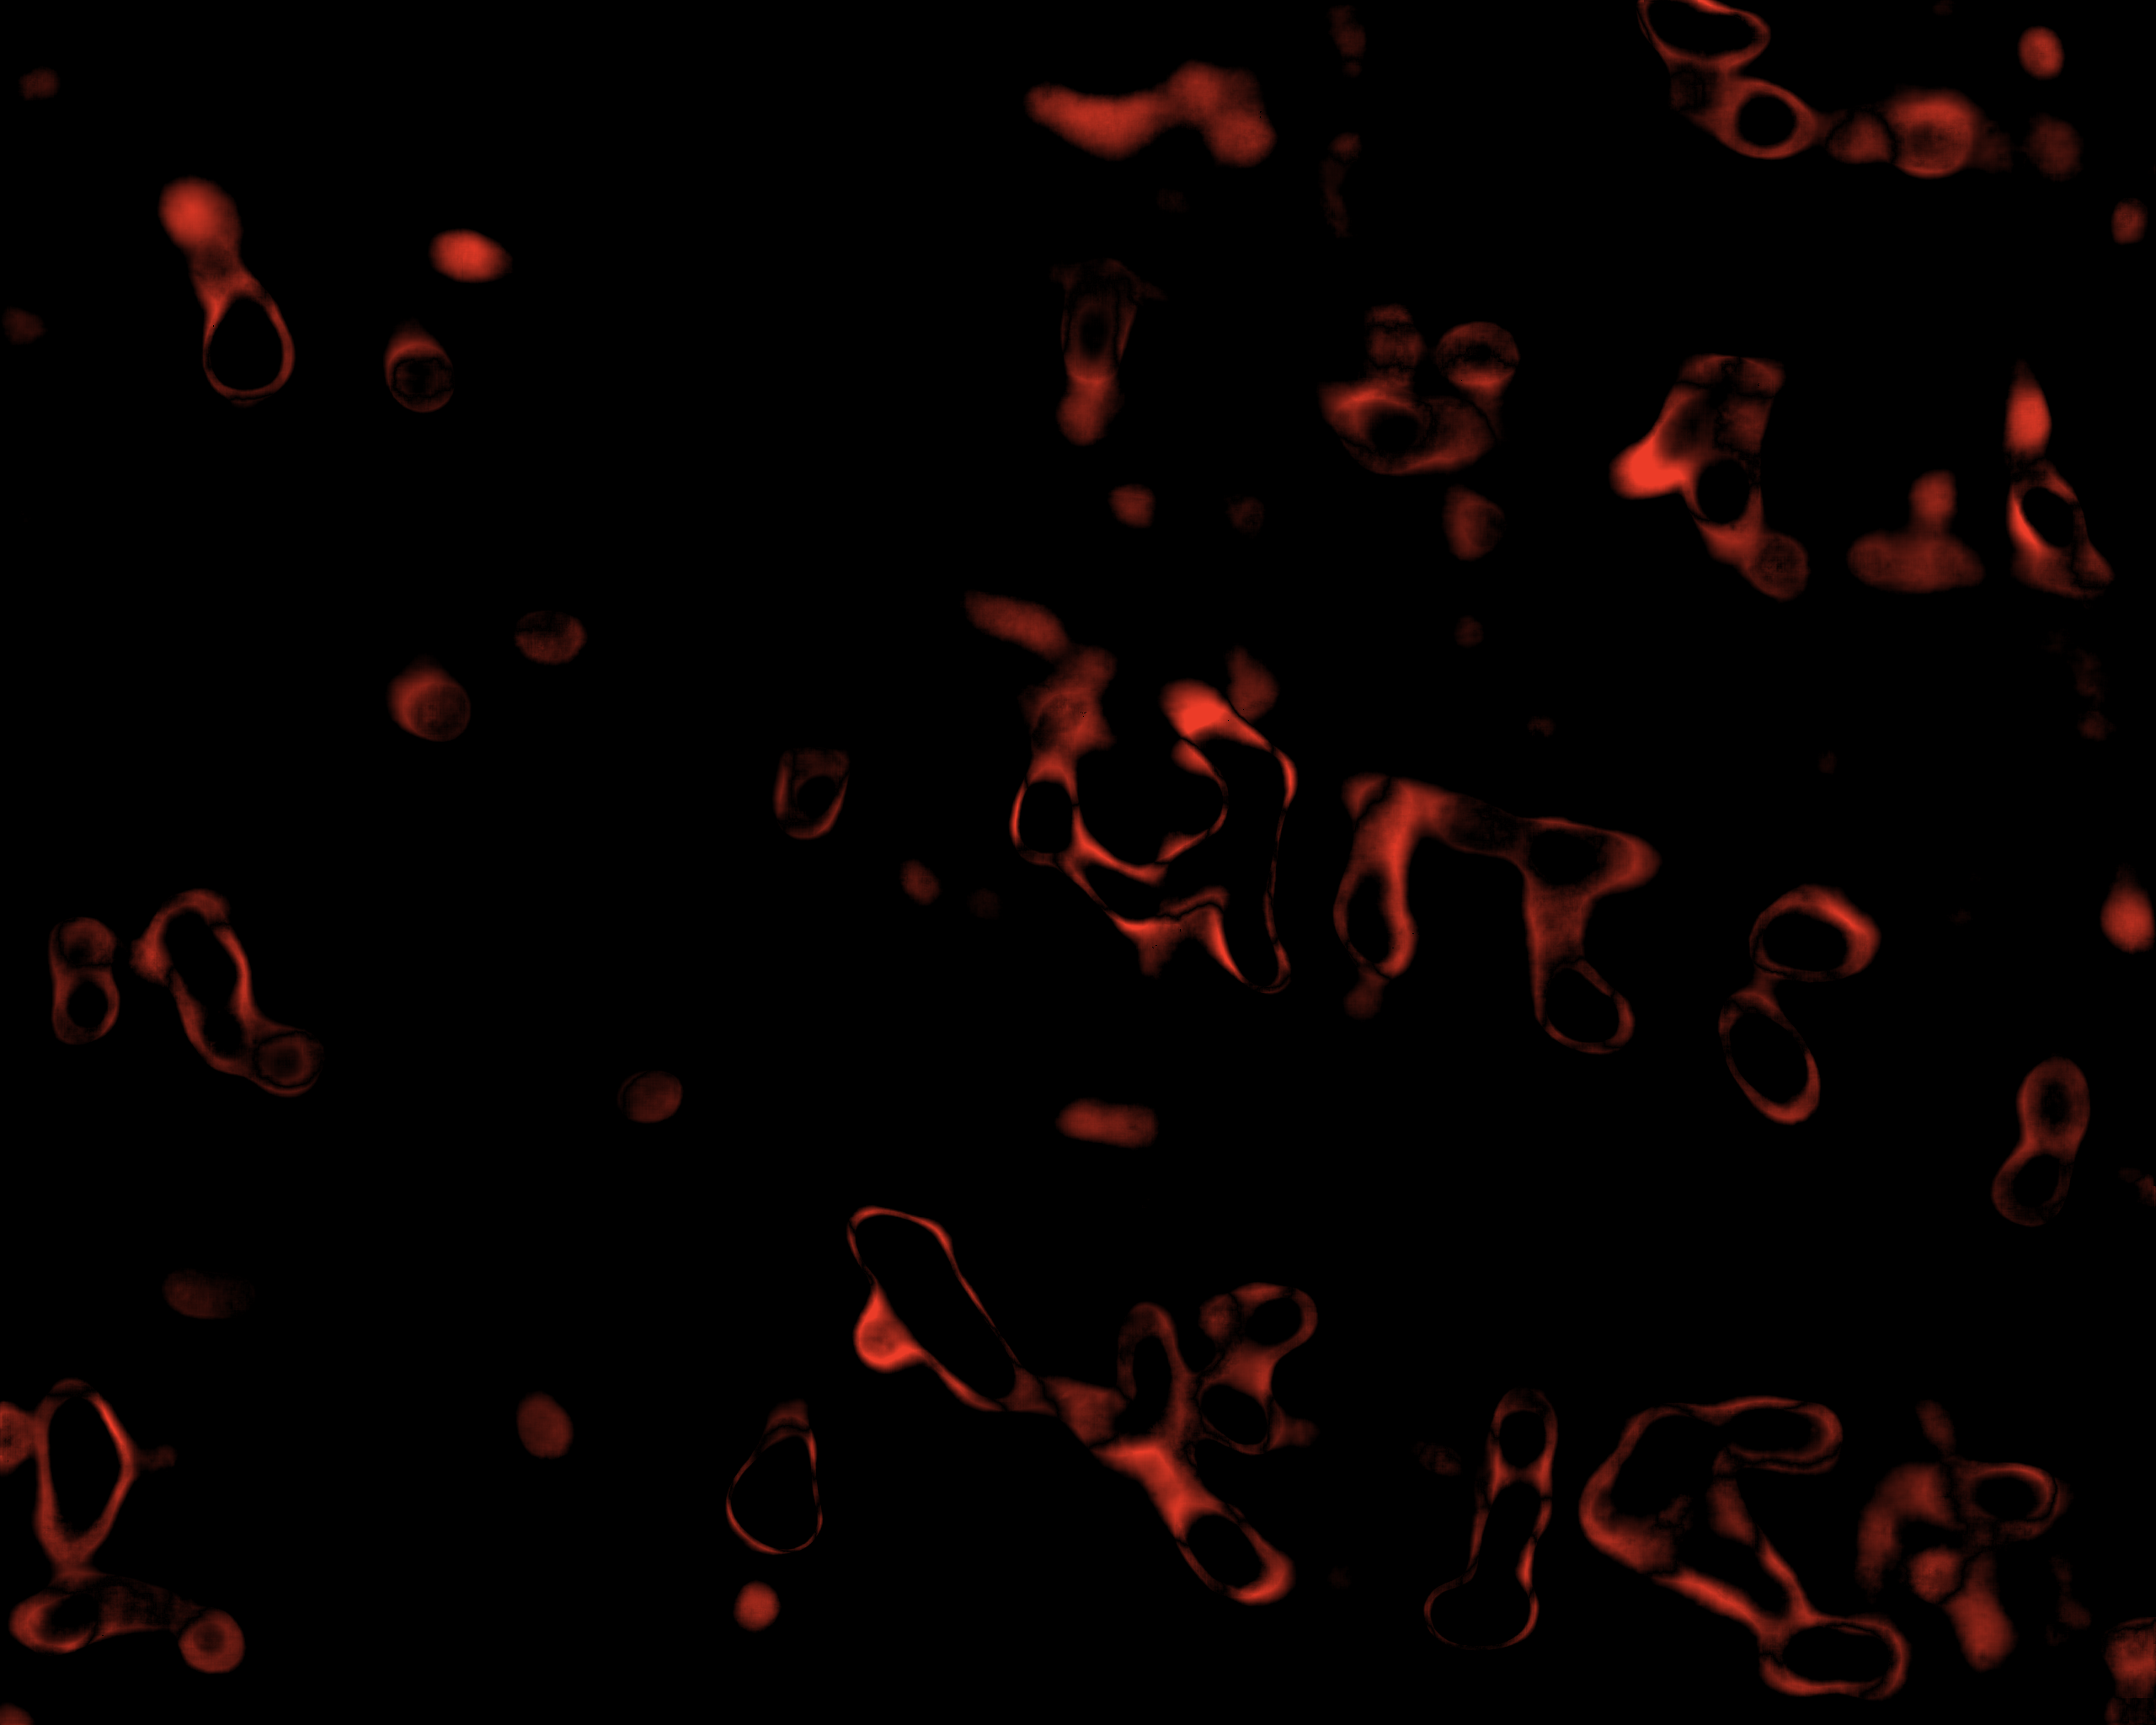
\includegraphics[width=0.29\textwidth]{../figures/m3/w00_3_difference.png}
\caption{Control unit 0841 w00. Left, Reader v3 (AUC 0.9055); centre, \MtName{} (AUC 0.8723); right, the red difference between the two maps. Each map is stretched between its own percentiles, the panels are shown at the full resolution of the file.}\label{fig:m3-w00}
\end{figure*}

\begin{figure*}[!tp]
\centering
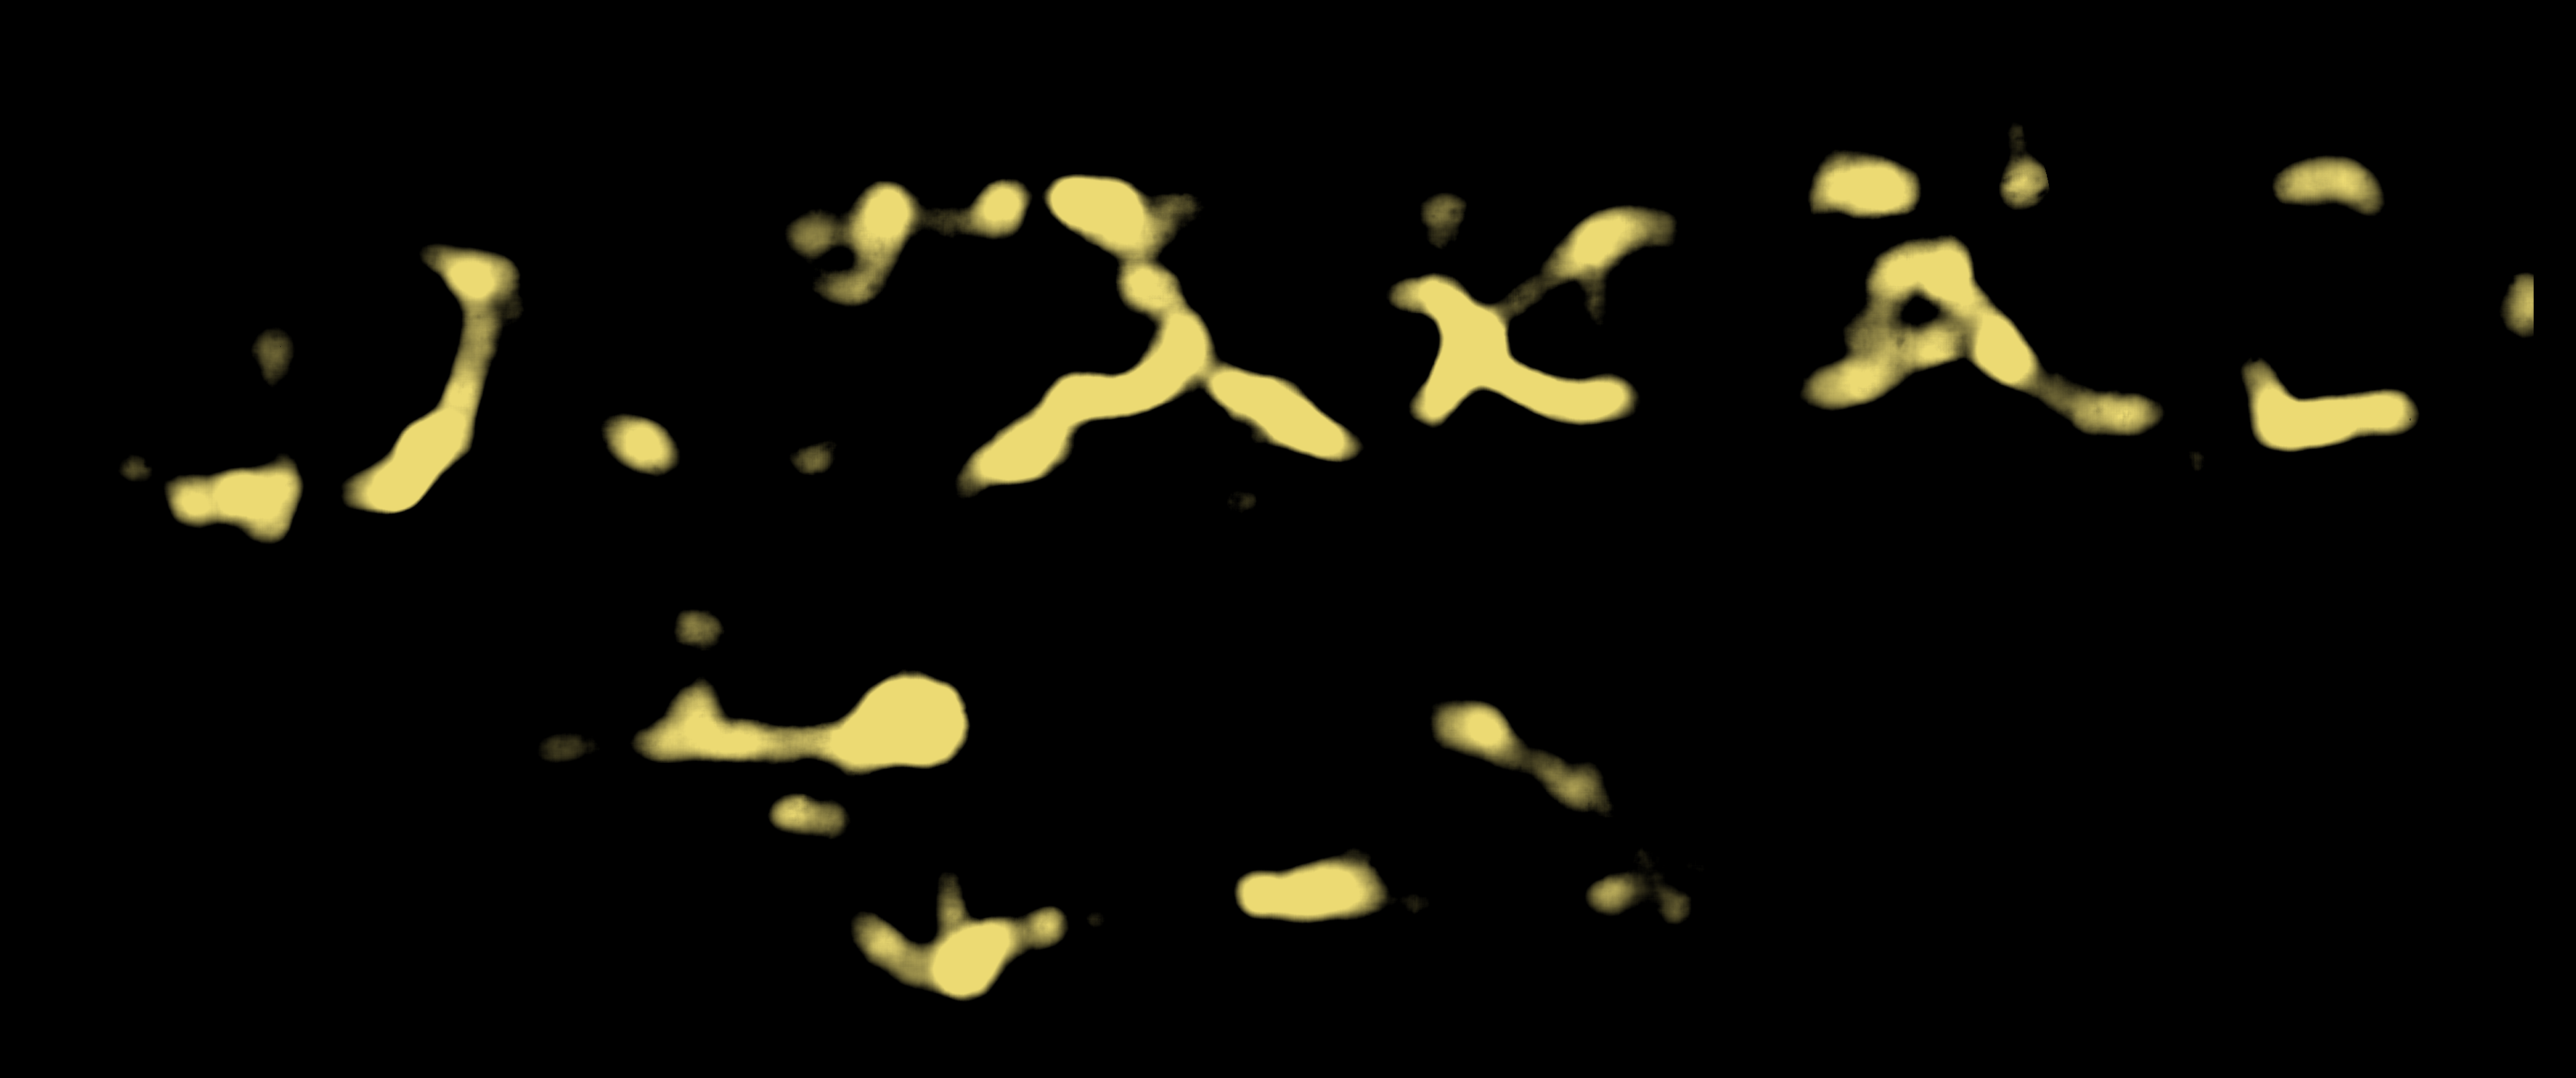
\includegraphics[width=0.29\textwidth]{../figures/m3/w058_1_reader-v3.png}
\hspace{3pt}
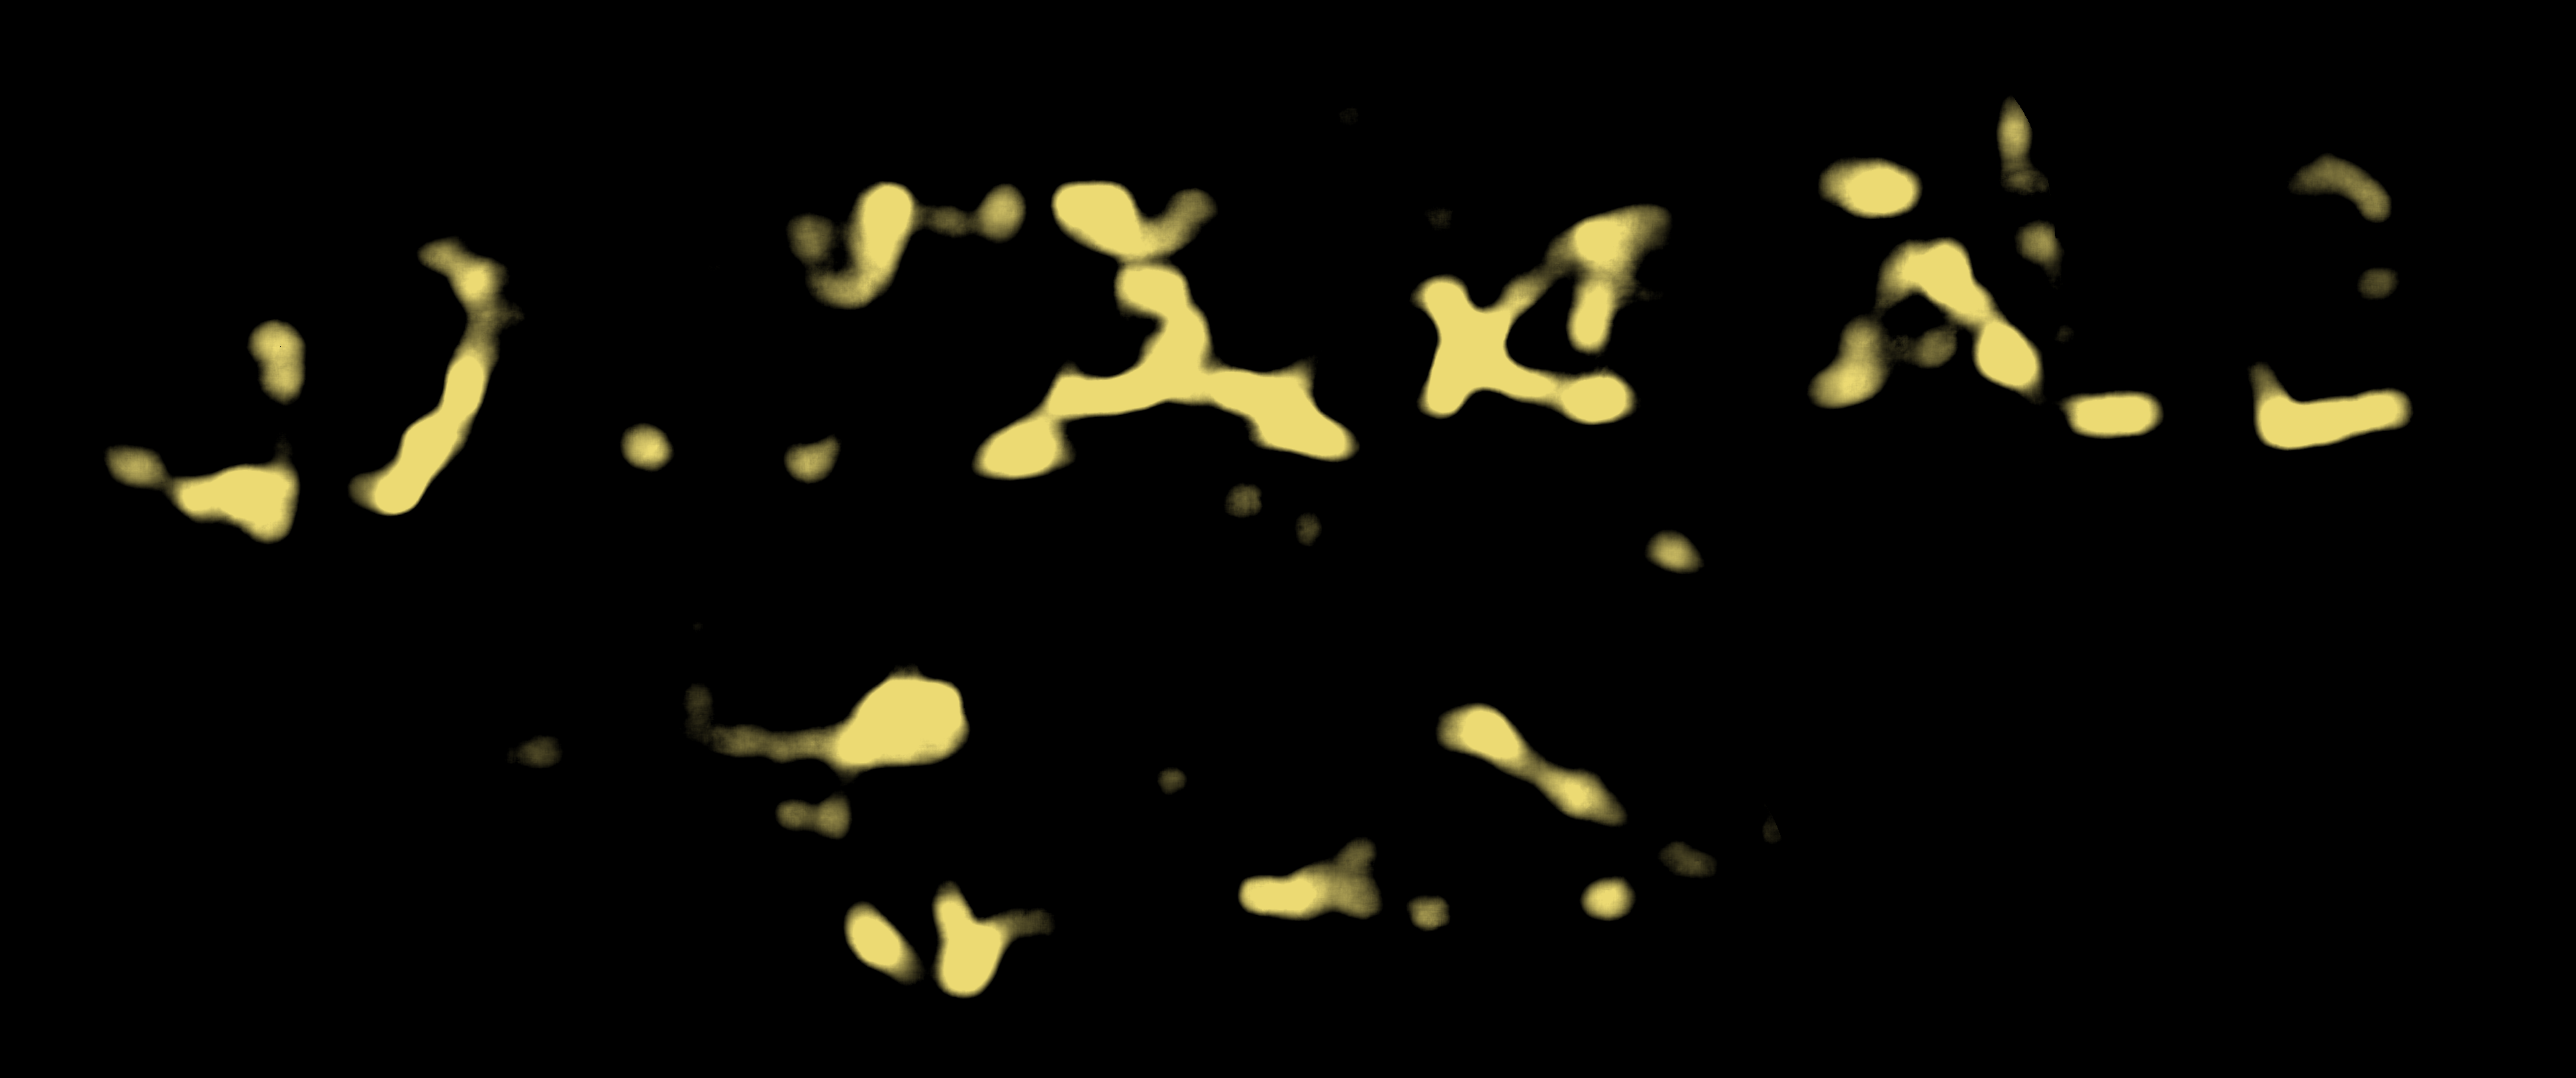
\includegraphics[width=0.29\textwidth]{../figures/m3/w058_2_m3.png}
\hspace{3pt}
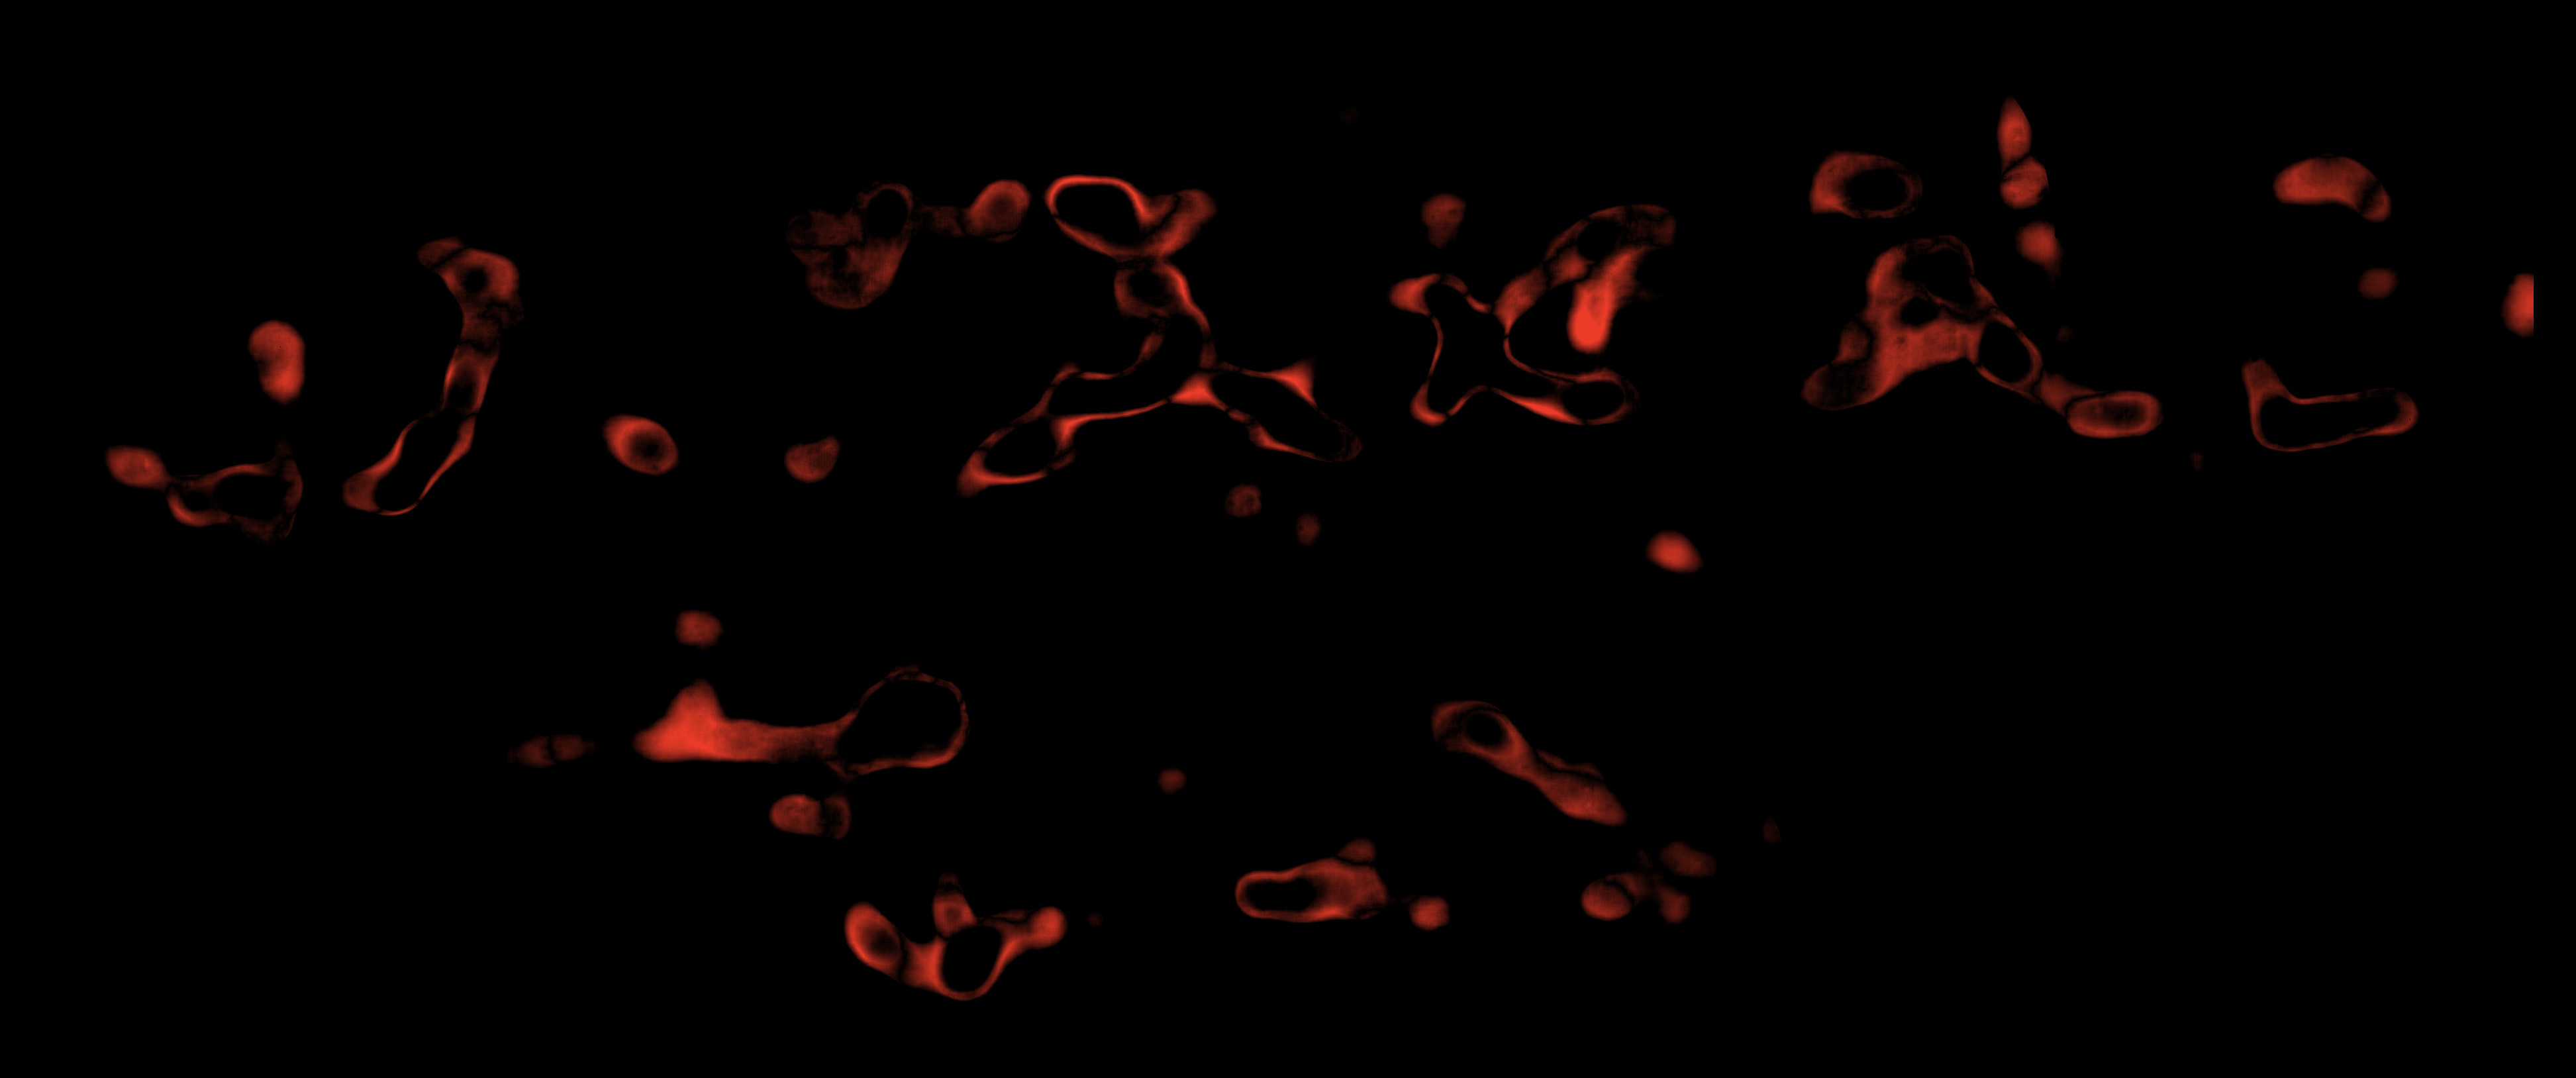
\includegraphics[width=0.29\textwidth]{../figures/m3/w058_3_difference.png}
\caption{Control unit 1447 w058. Left, Reader v3 (AUC 0.8610); centre, \MtName{} (AUC 0.8520); right, the red difference between the two maps. Each map is stretched between its own percentiles, the panels are shown at the full resolution of the file.}\label{fig:m3-w058}
\end{figure*}

\begin{figure*}[!tp]
\centering
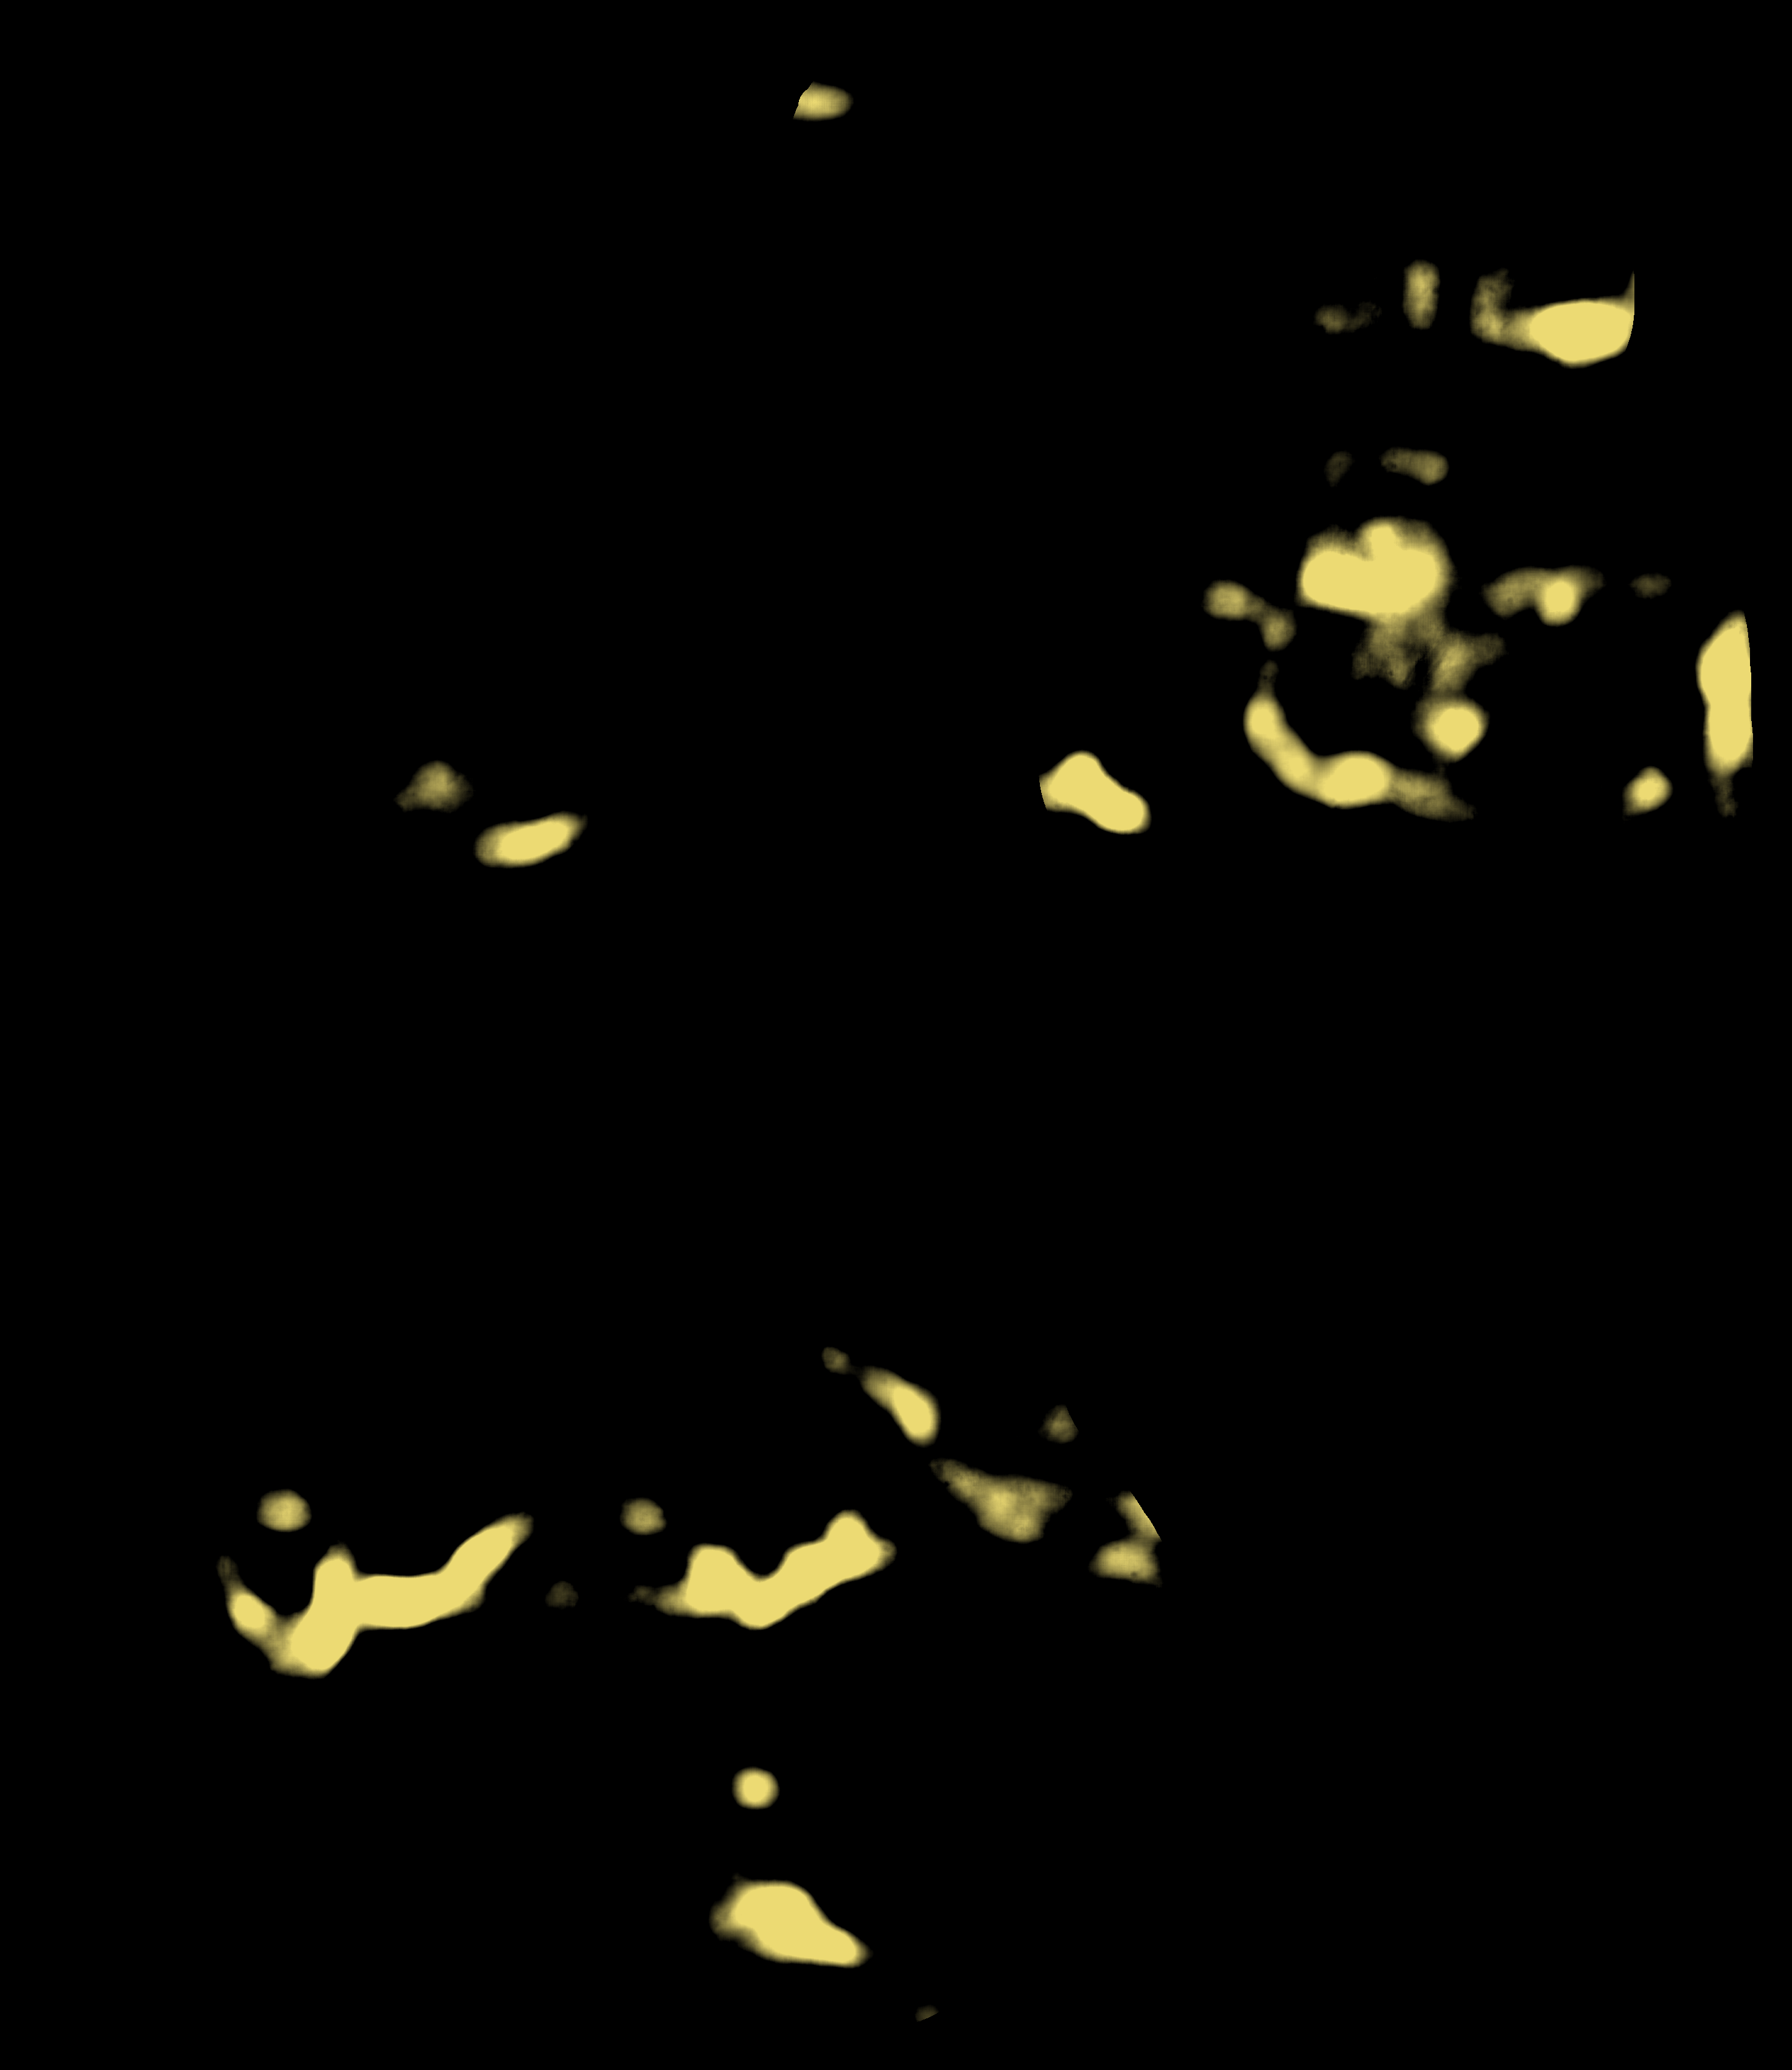
\includegraphics[width=0.29\textwidth]{../figures/m3/w060_1_reader-v3.png}
\hspace{3pt}
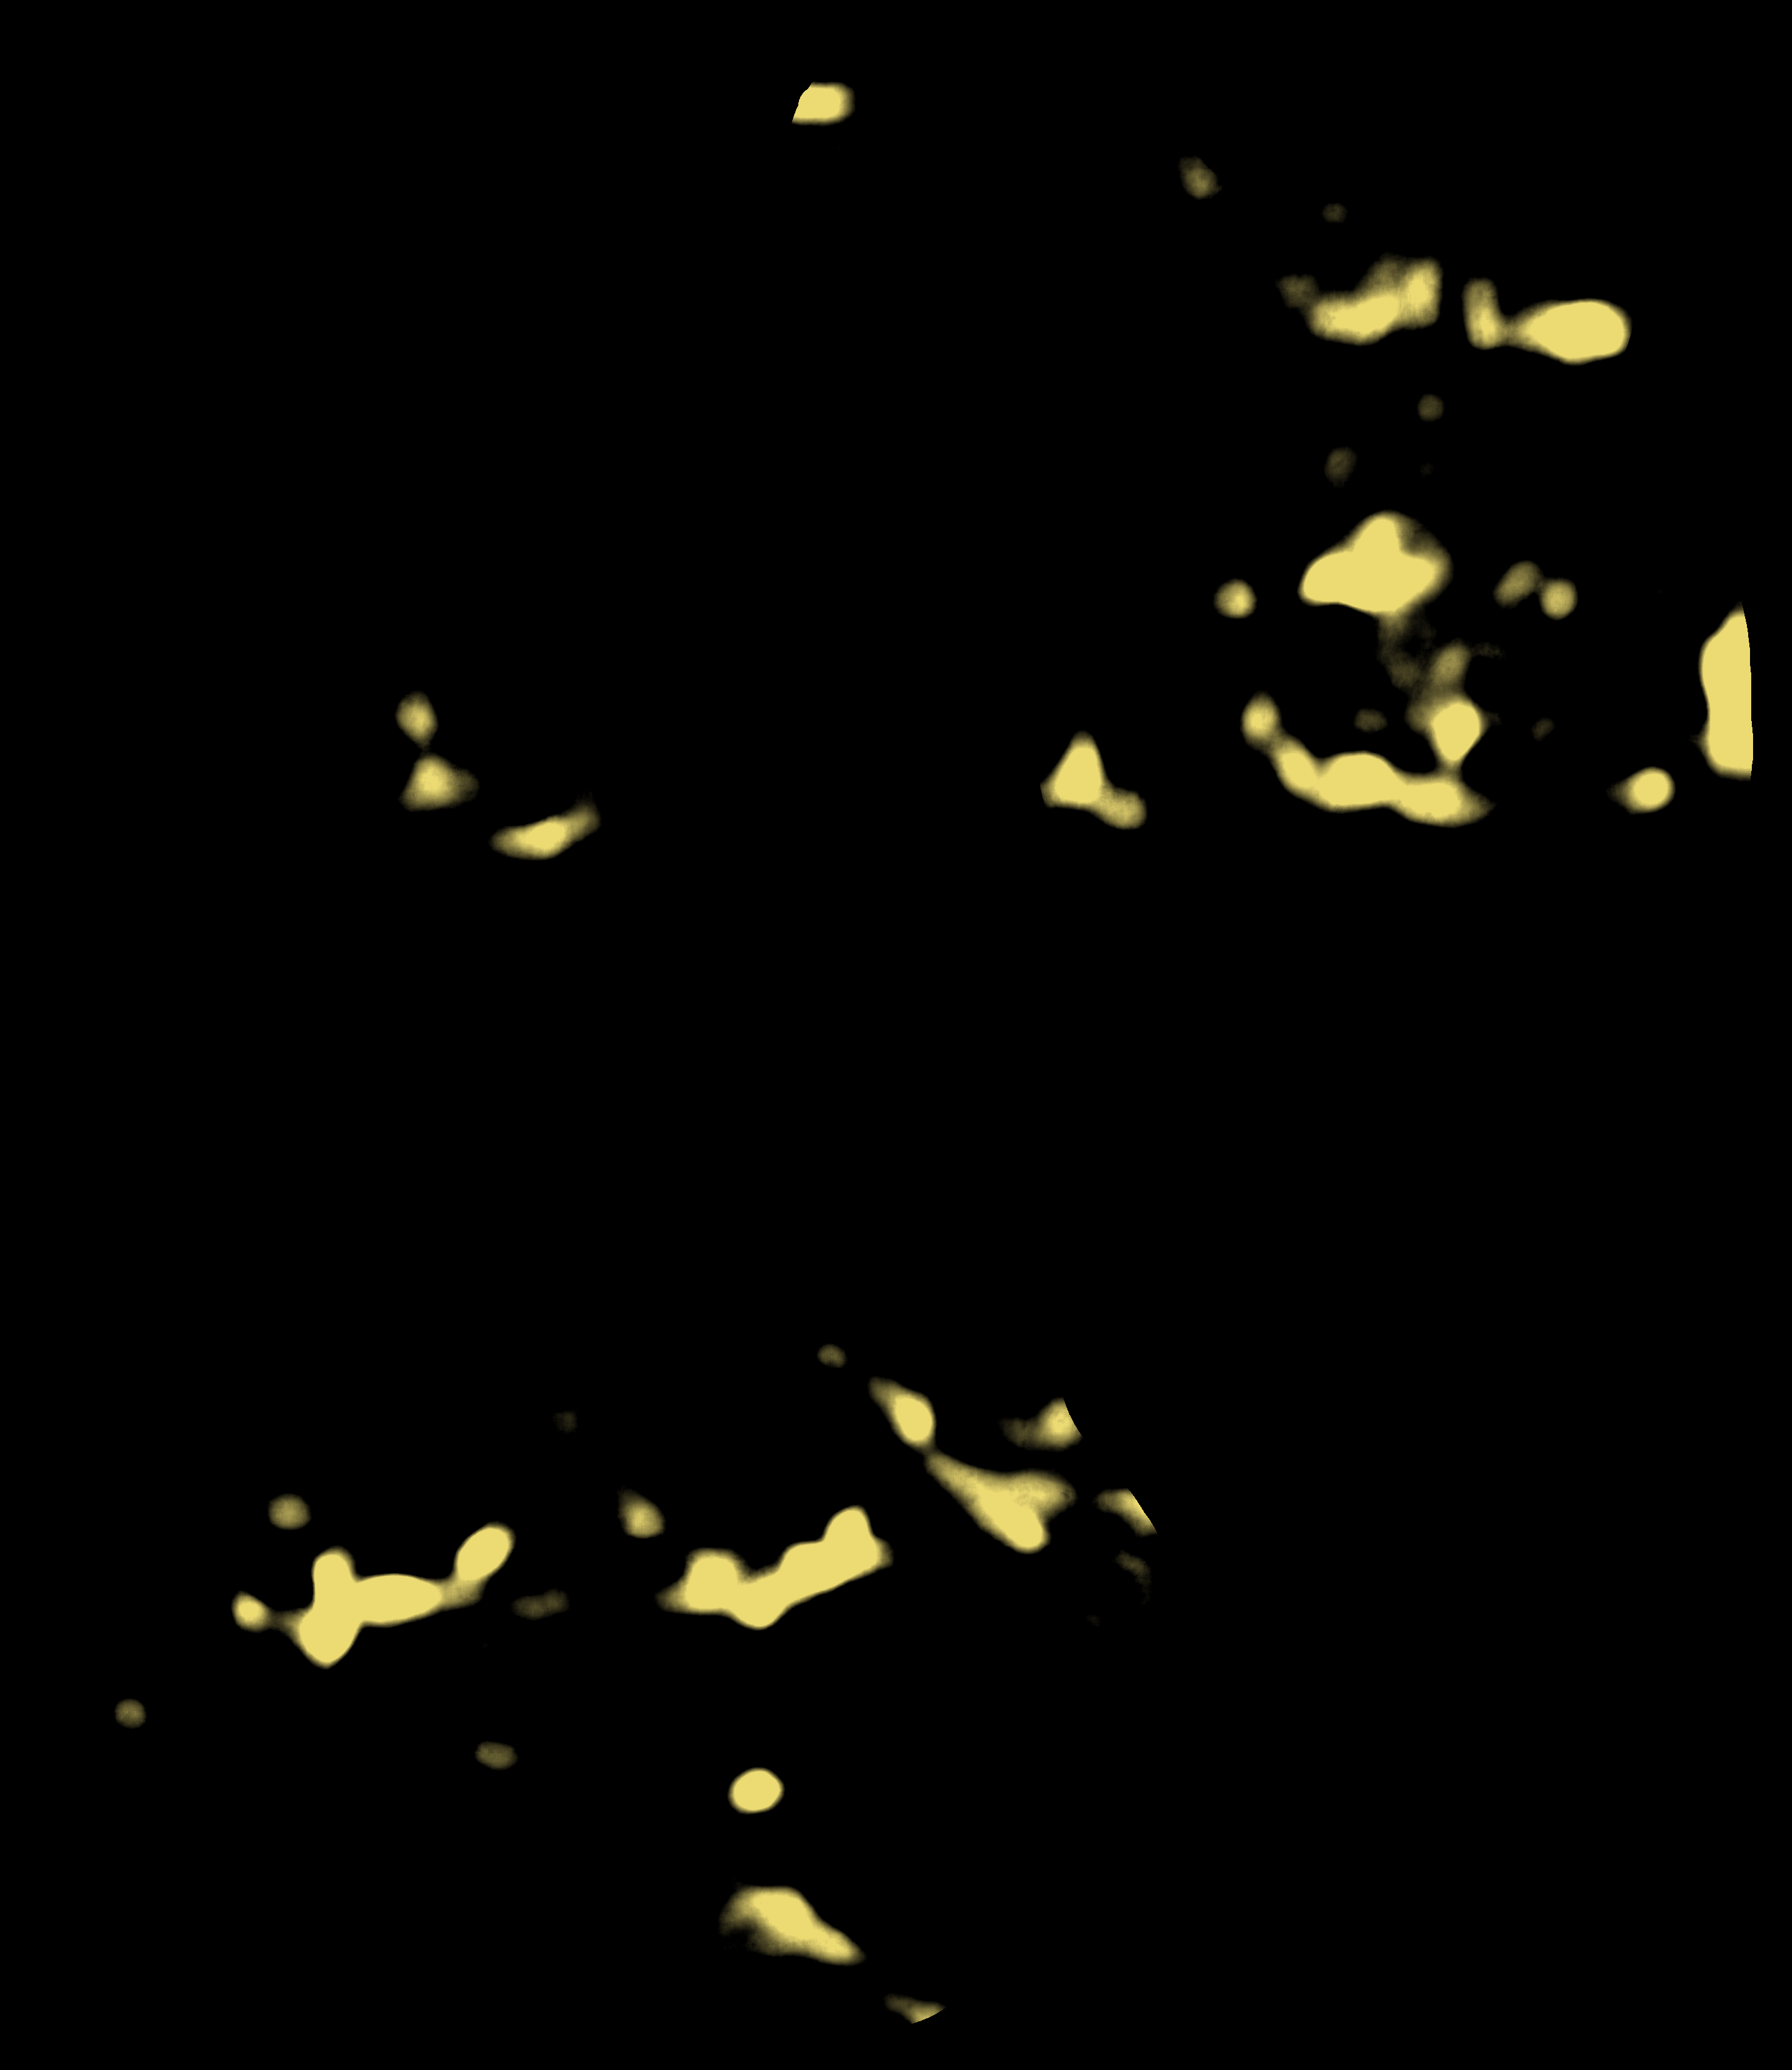
\includegraphics[width=0.29\textwidth]{../figures/m3/w060_2_m3.png}
\hspace{3pt}
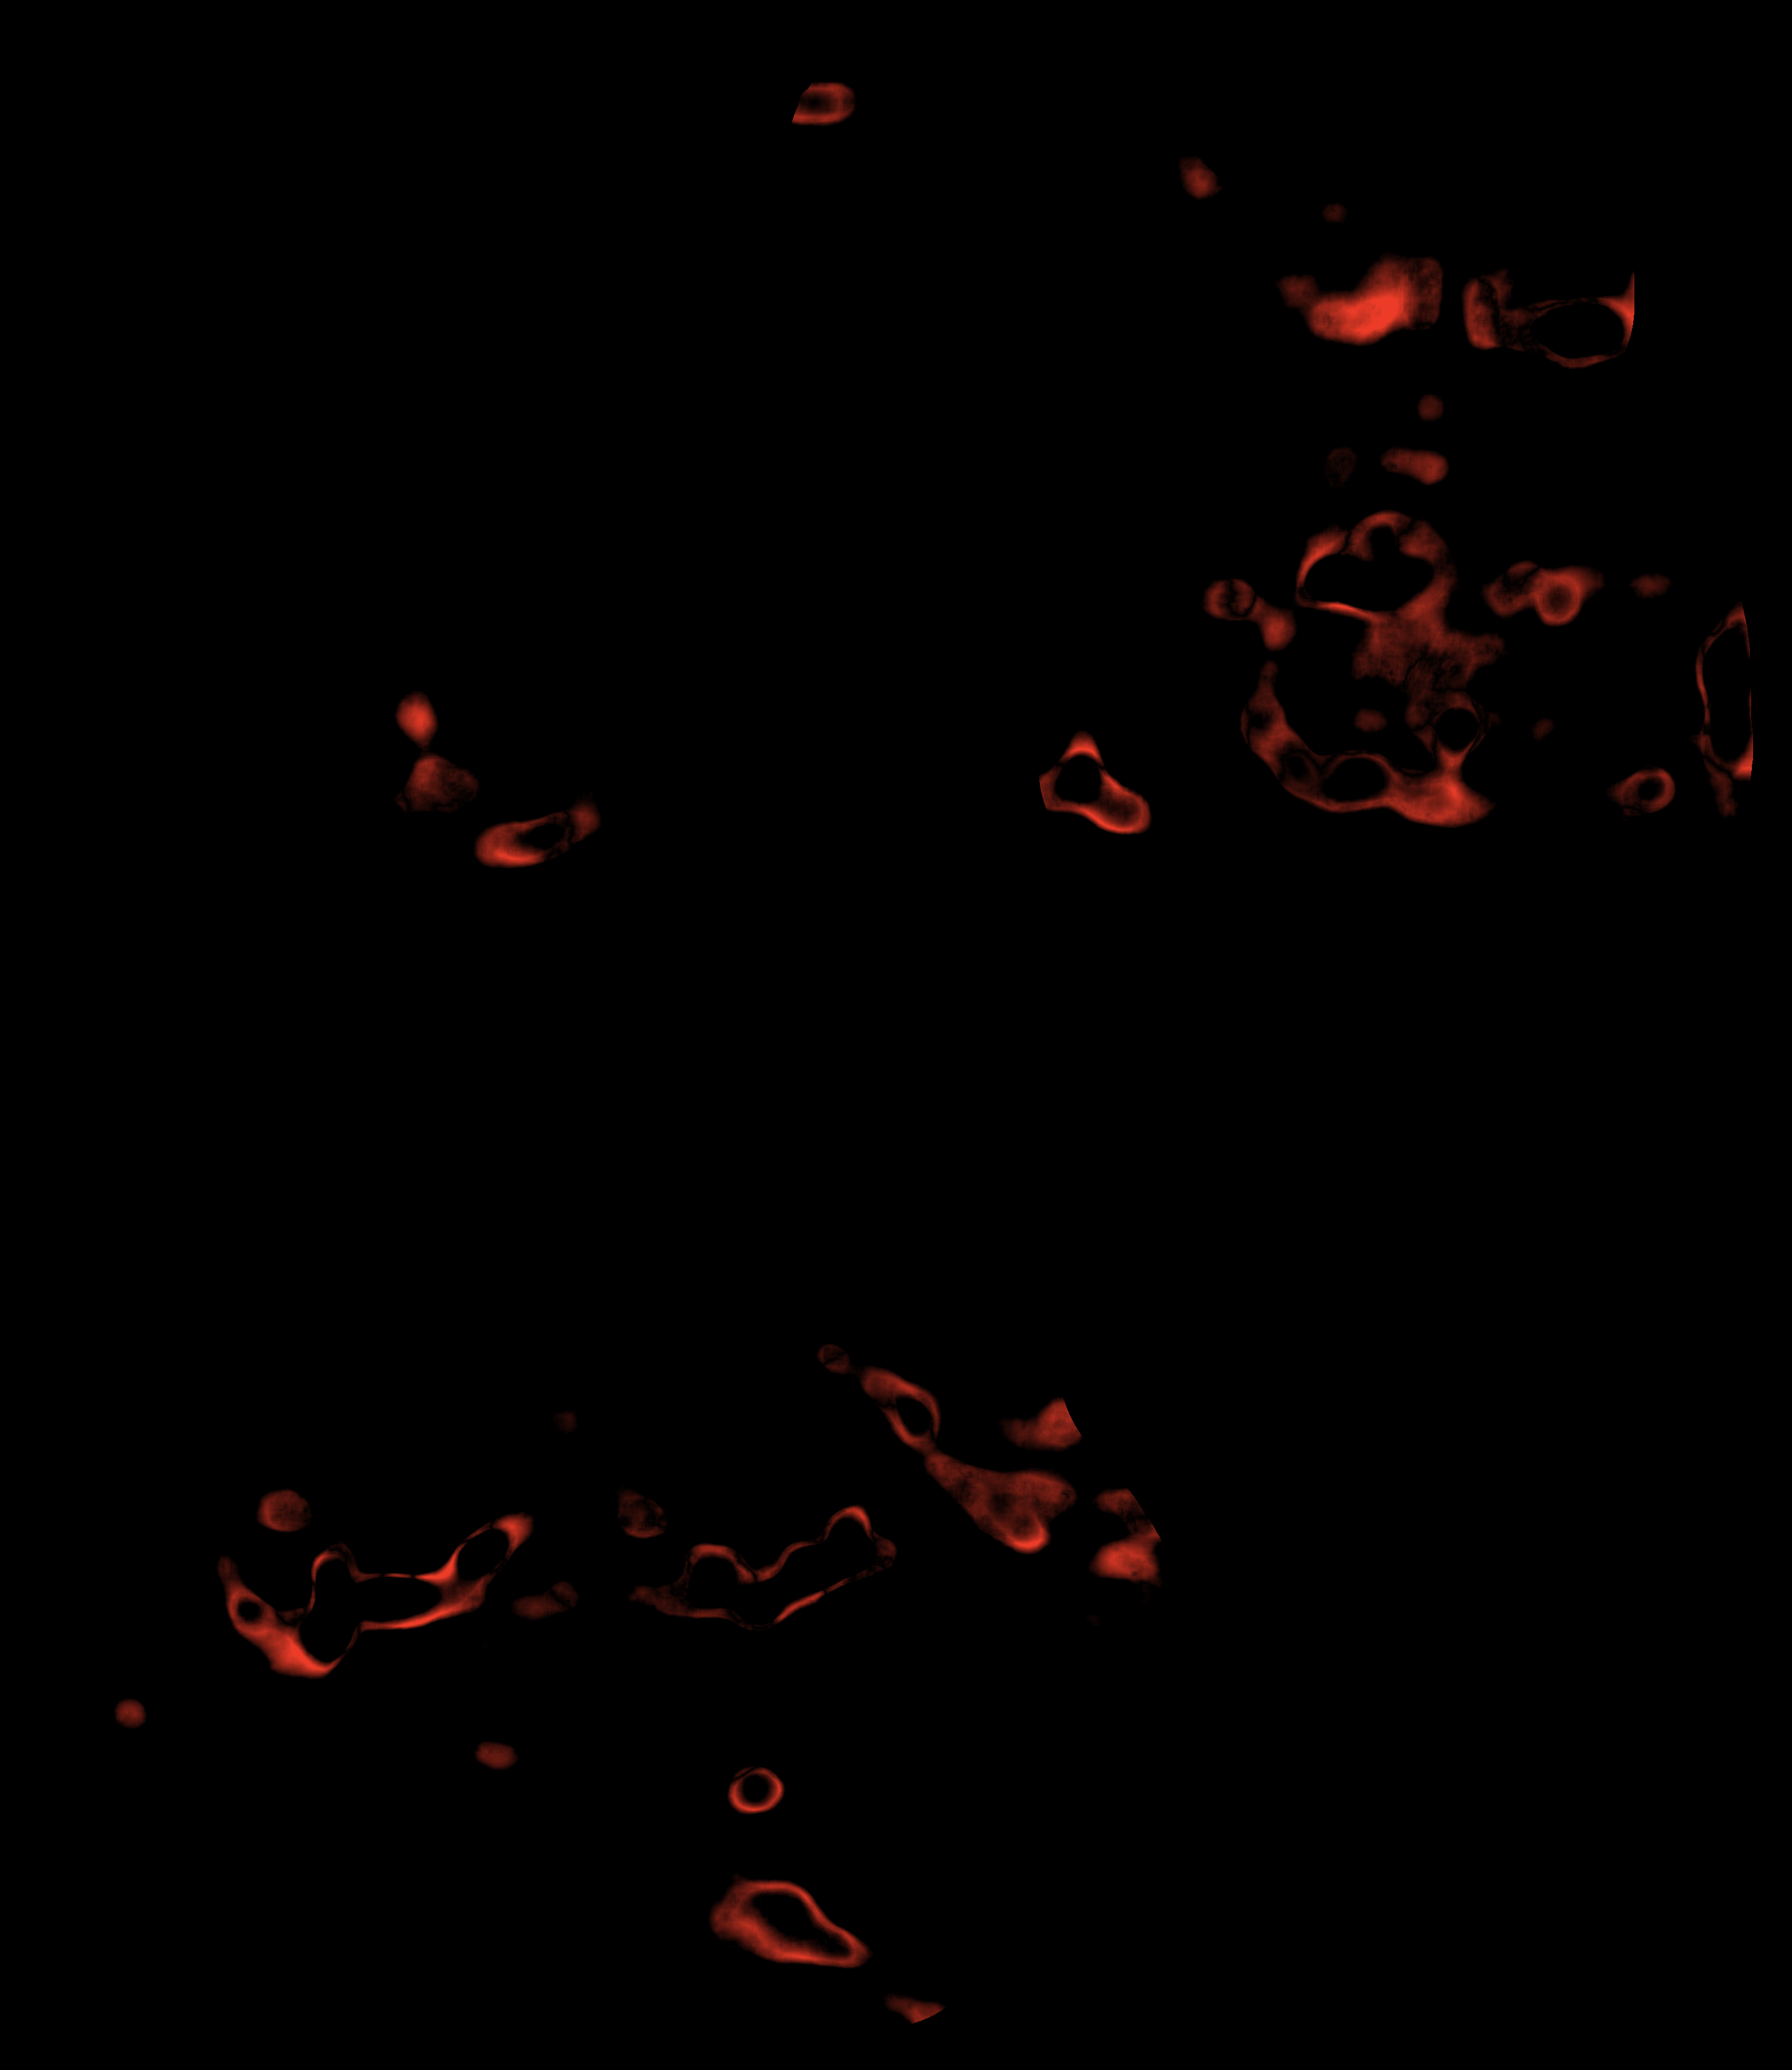
\includegraphics[width=0.29\textwidth]{../figures/m3/w060_3_difference.png}
\caption{Control unit 1447 w060. Left, Reader v3 (AUC 0.7842); centre, \MtName{} (AUC 0.7777); right, the red difference between the two maps. Each map is stretched between its own percentiles, the panels are shown at the full resolution of the file.}\label{fig:m3-w060}
\end{figure*}

